\documentclass[a4paper,12pt]{article}
\usepackage[numbib,nottoc,notlof]{tocbibind}
\usepackage{graphicx}
\usepackage{helvet}
\usepackage{wrapfig}
\usepackage[table]{xcolor}
\usepackage{geometry}
\usepackage{setspace}
\usepackage{float}
\usepackage{hyperref}
\usepackage{fancyhdr}
\usepackage{boldline}
\usepackage[labelfont=bf]{caption}
\usepackage{amsmath}

\renewcommand{\familydefault}{\sfdefault}
\renewcommand{\contentsname}{Index}
\renewcommand{\headrulewidth}{0pt}
\renewcommand{\footrule}{\hbox to\headwidth{\color{uoccyan}\leaders\hrule height \footrulewidth\hfill}}
\fancypagestyle{UOCfooterpage}{
    \fancyhf{}
    \renewcommand{\footrulewidth}{0.5pt}
    \fancyfoot[L]{\color{uocblue} Máster Universitario en Bioinformática y Bioestadística\hspace{2.2cm} 02/09/2022}
    }
\def\arraystretch{1.5}
\definecolor{uoccyan}{RGB}{115, 237, 255}
\definecolor{uocblue}{RGB}{0, 0, 120}
\definecolor{uocgrey}{RGB}{230, 230, 230}
\setlength\fboxsep{1cm}
\setlength{\parindent}{0pt}
\hypersetup{
    colorlinks=true,
    linkcolor=black,
    citecolor=black,
    urlcolor=blue
} 
\pagestyle{fancy}

%%%%%%%%%%%%%%%%%%%%%%%%%%%%%%%%%%%%%%%%%%%%%%%%%%%%%%%%%%%
% Customs
\newcommand{\thistitle}{Docking assays of Musashi-1 allosteric RNA-binding sites}
\newcommand{\thisauthor}{Lucas Goiriz Beltrán}
\newcommand{\thissupervisor}{Emmanuel Fajardo}
\newcommand{\thisPRA}{Emmanuel Fajardo}
\newcommand{\duedate}{12 de Enero 2023}
\newcommand{\duedateshort}{01/2023}
%%%%%%%%%%%%%%%%%%%%%%%%%%%%%%%%%%%%%%%%%%%%%%%%%%%%%%%%%%%


\begin{document}

%%%%%%%%%%%%%%%%%%%%%%%%%%%%%%%%%%%%%%%%%%%%%%%%%%%%%%%%%%%
%                       Title page                        %
%%%%%%%%%%%%%%%%%%%%%%%%%%%%%%%%%%%%%%%%%%%%%%%%%%%%%%%%%%%
\pagenumbering{gobble}
\newgeometry{left=2cm,right=1cm,top=2cm,bottom=0cm}

\colorbox{uoccyan}{\parbox{0.84\textwidth}{
    \setstretch{3}
    \vspace{1.2cm}
    \color{uocblue}\fontsize{40pt}{1cm}\textbf{\thistitle}
    \vspace{1cm}
}}

\vspace{1cm}

\begin{minipage}{\paperwidth}
    \begin{minipage}{0.35\paperwidth}
        
\includegraphics[width=6cm]{assets/UOC_UB_logos}
    \end{minipage}
    \hspace{0.001\paperwidth}
    \begin{minipage}{0.45\paperwidth}
        \fontsize{24pt}{1cm}\textbf{\thisauthor}\\
        
        \vspace{0.5cm}
        
        {\fontsize{24pt}{1cm}\selectfont MU Bioinf. i Bioest.\\
        Área de trabajo final}\\
        
        \vspace{0.5cm}
        
        \fontsize{24pt}{1cm}\textbf{Nombre Tutor/a de TF}\\

        \vspace{0.1cm}

        {\fontsize{21pt}{1cm}\selectfont \thissupervisor}\\

        \vspace{0.1cm}

        \fontsize{24pt}{1cm}\textbf{Profesor/a responsable de la asignatura}\\

        \vspace{0.1cm}

        {\fontsize{21pt}{1cm}\selectfont \thisPRA}\\

        \vspace{0.5cm}

        \fontsize{21pt}{1cm}\textbf{Fecha Entrega}\\

        \vspace{0.5cm}

        {\fontsize{21pt}{1cm}\selectfont \duedate}

        \vspace{2cm}
    \end{minipage}
\end{minipage}

\pagebreak

%%%%%%%%%%%%%%%%%%%%%%%%%%%%%%%%%%%%%%%%%%%%%%%%%%%%%%%%%%%
%                       License Page                      %
%%%%%%%%%%%%%%%%%%%%%%%%%%%%%%%%%%%%%%%%%%%%%%%%%%%%%%%%%%%

\restoregeometry

\fancyhead{
\includegraphics[width=\linewidth]{assets/UOC_header.png}}
\thispagestyle{UOCfooterpage}
~
\vfill
\begin{minipage}[l]{0.4\paperwidth}
    
\includegraphics{assets/license.png}\\
    Esta obra está sujeta a una licencia de Reconocimiento-NoComercial-SinObraDerivada \href{http://creativecommons.org/licenses/by-nc-nd/3.0/es/
        }{3.0 España de Creative Commons}    
\end{minipage}
\pagebreak

%%%%%%%%%%%%%%%%%%%%%%%%%%%%%%%%%%%%%%%%%%%%%%%%%%%%%%%%%%%
%                       Summary Page                      %
%%%%%%%%%%%%%%%%%%%%%%%%%%%%%%%%%%%%%%%%%%%%%%%%%%%%%%%%%%%

\pagenumbering{roman}

\section*{\centering FICHA DEL TRABAJO FINAL}
\begin{table}[h!]
    \centering
    \begin{tabular}{V{4}r|p{9cm}V{4}}
        \hlineB{4}
        \textbf{Título del trabajo:} & \cellcolor{uocgrey}\textit{\thistitle}\\
        \hline
        \textbf{Nombre del autor:} & \cellcolor{uocgrey}\textit{\thisauthor}\\
        \hline
        \textbf{Nombre del consultor/a:} & \cellcolor{uocgrey}\textit{\thissupervisor}\\
        \hline
        \textbf{Nombre del PRA:} & \cellcolor{uocgrey}\textit{\thisPRA}\\
        \hline
        \textbf{Fecha de entrega:} & \cellcolor{uocgrey}\textit{\duedateshort}\\
        \hline
        \textbf{Titulación o programa:} & \cellcolor{uocgrey}\textit{Máster Universitario en Bioinformática y Bioestadística}\\
        \hline
        \textbf{Área del Trabajo Final} & \cellcolor{uocgrey}\textit{Drug Design and Structural Biology}\\
        \hline
        \textbf{Idioma del trabajo:} & \cellcolor{uocgrey}\textit{Inglés}\\
        \hline
        \textbf{Palabras clave:} & \cellcolor{uocgrey}\textit{Molecular Docking, RNA-binding protein, Allosteric Regulation}\\
        \hline\hline
        \multicolumn{2}{V{4}l V{4}}{\textbf{Resumen del Trabajo}}\\
        \hline
        \multicolumn{2}{V{4}p{14.3cm}V{4}}{\cellcolor{uocgrey} Máximo 250 palabras, con la finalidad, contexto de aplicación, metodología, resultados y conclusiones del trabajo}\\
        \hline
        \multicolumn{2}{V{4}l V{4}}{\textbf{Abstract}}\\
        \hline
        \multicolumn{2}{V{4}p{14.3cm}V{4}}{\cellcolor{uocgrey} A maximum of 250 words, detailing the purpose, context of application, methodology, results and conclusions of the work}\\
        \hlineB{4}
    \end{tabular}
\end{table}
\pagebreak

%%%%%%%%%%%%%%%%%%%%%%%%%%%%%%%%%%%%%%%%%%%%%%%%%%%%%%%%%%%
%                     Section Index Page                  %
%%%%%%%%%%%%%%%%%%%%%%%%%%%%%%%%%%%%%%%%%%%%%%%%%%%%%%%%%%%

\tableofcontents

\pagebreak

%%%%%%%%%%%%%%%%%%%%%%%%%%%%%%%%%%%%%%%%%%%%%%%%%%%%%%%%%%%
%                      Figure Index Page                  %
%%%%%%%%%%%%%%%%%%%%%%%%%%%%%%%%%%%%%%%%%%%%%%%%%%%%%%%%%%%

\listoffigures

\pagebreak

%%%%%%%%%%%%%%%%%%%%%%%%%%%%%%%%%%%%%%%%%%%%%%%%%%%%%%%%%%%
%                          Sections                       %
%%%%%%%%%%%%%%%%%%%%%%%%%%%%%%%%%%%%%%%%%%%%%%%%%%%%%%%%%%%

% La memoria debería ocupar entre 30 y 60 páginas. Esta cifra es orientativa y no debería limitaros. En cualquier caso, la memoria no puede ocupar más de 90 páginas (sin tener en cuenta los anexos).

\pagenumbering{arabic}

% Section 1: Introduction
\section{Introduction}

\subsection{Context and justification}

The Musashi-1 (MSI-1) protein belongs to a family of neural RNA-binding proteins (RBPs) that play a fundamental role in neural development in both vertebrates and invertebrates \cite{nakamura_1994,sakakibara_1996, good_1998, imai_2001}. In particular, the mouse MSI-1 consists of 362 aminoacids with a molecular mass of 39 kDa \cite{sakakibara_1996}, and contains 2 sequences of around 80 to 90 aminoacids that interact with RNA (RRMs; short for RNA-recognition motifs) following the consensus sequence \texttt{RU}$_n$\texttt{AGU}\footnote{Following the IUPAC standard for degenerate base symbols, \texttt{R} represents both an Adenine (\texttt{A}) and a Guanine (\texttt{G}). Refer to \cite{cornish_1985} for the complete IUPAC standard.}$^,$\footnote{\texttt{U}$_n$ stands for repeating \texttt{U} within the consensus sequence $n$ times. In most cases, $n\in\left\{1,2,3\right\}$ \cite{imai_2001}.} \cite{imai_2001,zearfoss_2014}.\\

Despite multiple efforts, the complete structure of any of the MSI-1 protein homologues remains a mystery. The most notable successes have only been able to completely elucidate MSI-1's RRM1 and RRM2 domains \cite{nagata_1999,miyanoiri_2003,ohyama_2011,lan_2019}, see for example \textbf{Figure \ref{fig:3DRRM1}} for the 3D structure of RRM1. 

\begin{figure}[htbp!]
    \centering
    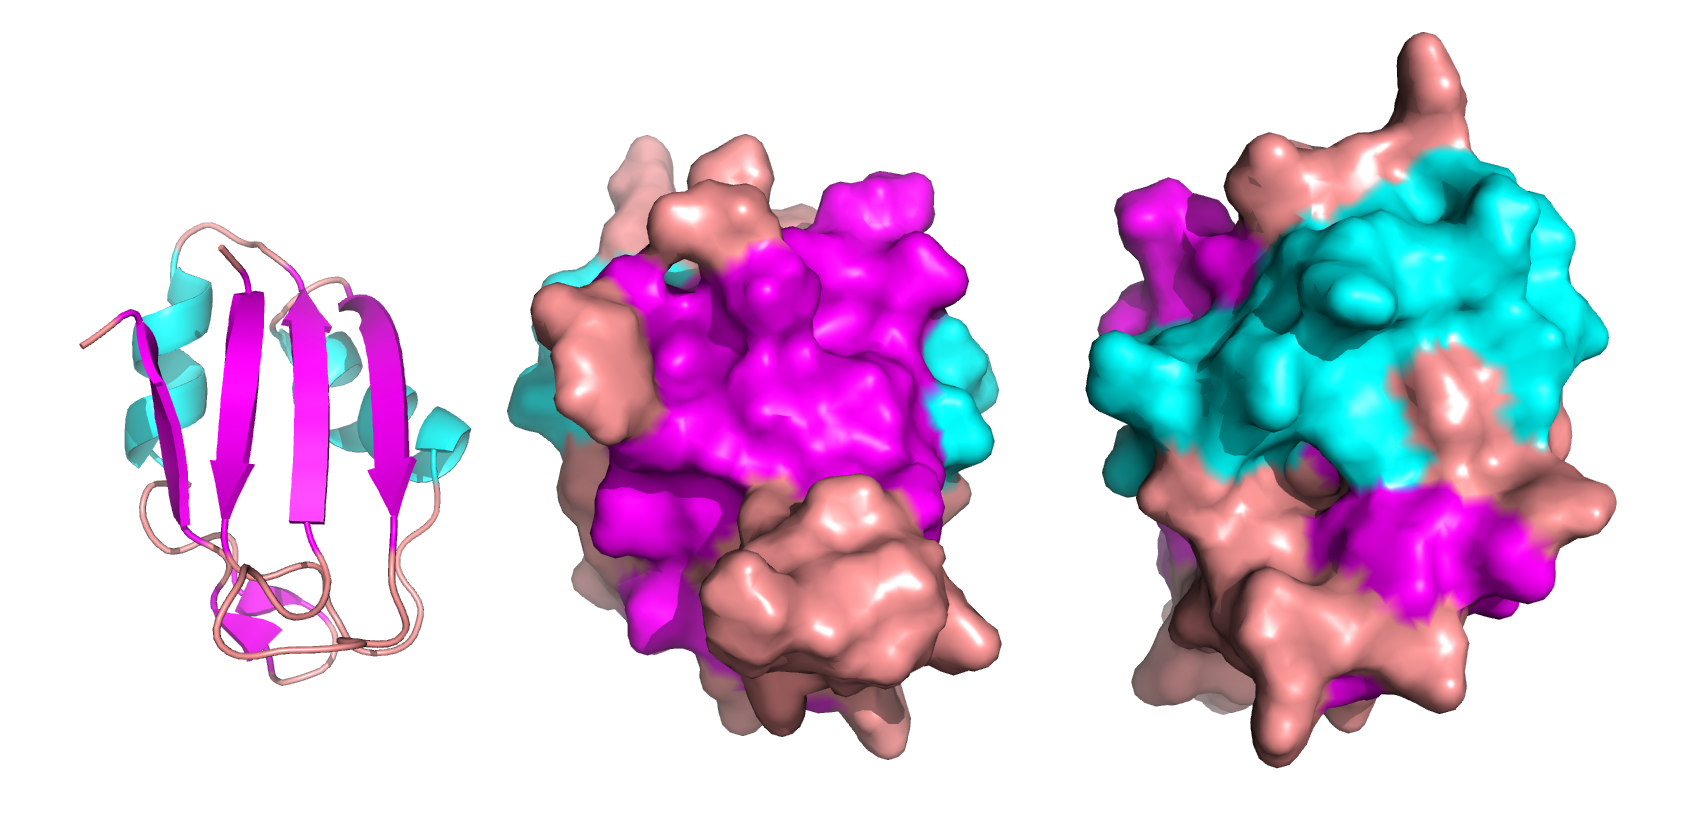
\includegraphics[width=0.9\linewidth]{assets/RRM1_various.png}
    \caption[3D RRM1 structure of the MSI-1 protein constructred by means of protein crystalization and RMN.]{3D RRM1 structure of the MSI-1 protein constructred by means of protein crystalization and RMN. From left to right: RRM1 in \textit{cartoon} setting, RRM1 in \textit{surface} setting and RRM1 in \textit{surface} setting turned 180$^\circ$. Colors represent the secondary structures found within the protein: cyan corresponds to $\alpha$-helices, magenta corresponds to $\beta$-sheets and salmon corresponds to \textit{random coil}. The model was retrieved from \href{https://www.uniprot.org/uniprotkb/Q61474/entry}{\texttt{Uniprot} entry \texttt{Q61474}}. Visualized through \href{https://pymol.org/2/}{\texttt{Pymol}}.}
    \label{fig:3DRRM1}
\end{figure}

\pagebreak

At the moment, the available complete MSI-1 structures only originate from computational predictions, such as the one shown in \textbf{Figure \ref{fig:3DMSI}} which is an aminoacid-sequence-based prediction yielded by \href{https://alphafold.ebi.ac.uk/}{\texttt{AlphaFold}} \cite{jumper_2021}.

\begin{figure}[htbp!]
    \centering
    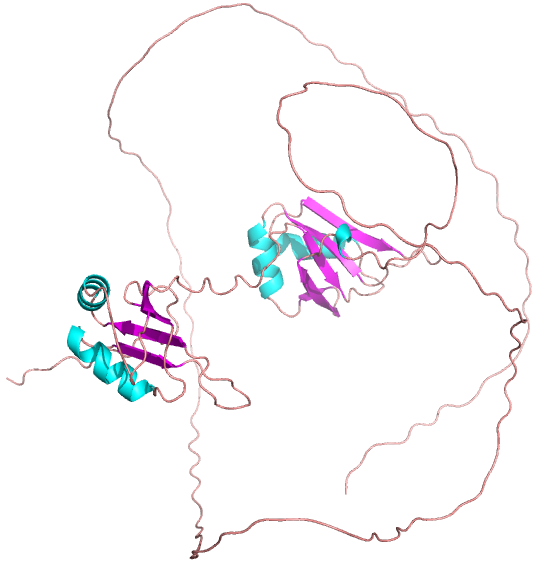
\includegraphics[width=0.5\linewidth]{assets/MSI1_complete.png}
    \caption[3D mouse MSI-1 structure as predicted by \texttt{AlphaFold}.]{3D mouse MSI-1 structure as predicted by \href{https://alphafold.ebi.ac.uk/}{\texttt{AlphaFold}}, in \textit{cartoon} setting. Colors represent the secondary structures found within the protein: cyan corresponds to $\alpha$-helices, magenta corresponds to $\beta$-sheets and salmon corresponds to \textit{random coil}. The model was retrieved from \href{https://www.uniprot.org/uniprotkb/Q61474/entry}{\texttt{Uniprot} entry \texttt{Q61474}}. Visualized through \href{https://pymol.org/2/}{\texttt{Pymol}}.}
    \label{fig:3DMSI} 
\end{figure}

With the surge of synthetic biology during the past two decades, RBPs such as MSI-1 have gained a special interest for their applicability as post-transcriptional regulators of gene expression in synthetic gene circuits \cite{belmont_2010,cao_2015,katz_2019}. In particular, Dolcemascolo and colleagues pioneered by designing a synthetic genetic circuit employing MSI-1 as post-transcriptional regulator \cite{dolcemascolo_2022}. In addition, they also exploited MSI-1's particularity of binding to fatty acids in addition to RNA, out of which the cis-9-Octadecenoic acid (also known as oleic acid) presents a higher binding affinity. The latter interaction weakens the MSI-1 protein's RNA-binding affinity, resulting in a dissociation between MSI-1 and the RNA sequence \cite{dolcemascolo_2022,clingman_2014}. In fact, the pocket in which the fatty acids interact with the RMM1 domain of MSI1 can be easily seen in the rightmost protein in \textbf{Figure \ref{fig:3DRRM1}}.\\

Therefore, in order to confidently add MSI-1 as an allosteric regulator to the synthetic biologist's toolbox, there is a need to understand how the underlying interaction mechanisms work. Clingman and colleagues are were the first who performed docking simulations with the MSI-1 core RNA-binding-motif and several fatty acids \cite{clingman_2014}. Nevertheless, these results only hold for the aforementioned RNA-motif: it is expected that any mutation on the RNA-motif would drastically impact the manner in which MSI-1 interacts with the RNA.

\subsection{Objectives}

This Master's Thesis aims to extend the knowledge behind the allosteric interactions occurring in the MSI-1 proteins by performing docking simulations between MSI-1's RRM1 domain, several RNA motifs and fatty acids, with the objective of obtaining a model for each of the combinatorial cases.\\

This general objective breaks down into the following specific objectives:

\begin{enumerate}
    \item \textit{In silico} Generate the 3D structures of 5 mutant MSI-1 RNA-binding motifs used in \cite{dolcemascolo_2022}. The 3D structures of the motifs will depend on the sequence-based-prediction of their secondary structures.
    \item Assess the structure of MSI-1's RRM1-RNA mutant complex through docking for each of the mutants.
    \item Assess the structure of MSI-1's RRM1-fatty acid complex through docking for each of the fatty acids of interest: oleic acid, linoleic acid, palmitoleic acid, arachidonic acid and stearic acid.
    \item Keep the top 2 fatty acids whose interaction with MSI-1 is the clearest.
    \item Assess the structure of RNA mutant-MSI-1's RRM1-fatty acid complex through the coupling of the docking models obtained.
\end{enumerate}
    
\subsection{Impact on sustainability, social-ethical and diversity}

\subsubsection{Sustainability}

The result of this Master's Thesis has had a negligible but negative impact on sustainability. This impact originates on the energy consumption during the following steps:

\begin{enumerate}
    \item Design and debugging of the docking pipeline followed in this work.
    \item Computation of the different models.
\end{enumerate}

This impact can be considered negligible because the net amount of energy consumed during the computations is very small. Nevertheless, it is important to highlight this aspect as there is room for improvement: the source code of the docking software employed in this work is mainly composed of two programming languages: \texttt{C} (72\%) and \texttt{Python} (28\%).\\

Pereira and colleagues developed a benchmark to order programming\linebreak languages with respect of their energy consumption when executing well-known computer science algorithms and data structures \cite{pereira_2017}. Their finding was that the least energy consuming programming language was \texttt{C}, while \texttt{Python} was one of the most energy consuming.\\

It can be discussed that, in order to reach minimal energy consumption, the programming language to be used in software that is going to be distributed and executed multiple times should be exclusively \texttt{C}. The disadvantages of \texttt{C} are that it takes more time to write a full program than with higher level languages (such as \texttt{Python}), it is more difficult to mantain a codebase written in \texttt{C} and that \texttt{C} is not a particularly accessible programming language for non-computer scientists.\\

There is a trade-off that has be to be considered. Let $L$ be a programming language, $E_{W_L}$ be the energy consumed by a computer during the crafting of a software written in $L$, $E_{E_L}$ be the energy consumed by a computer during one execution of the software written in $L$ (in this particular case, one docking simulation with some fixed parameters) and $n$ be the number of times the software is executed, then it is possible to approximate $E_{T_L}(n)$ (the total energy consumed by the software written in $L$ at the moment $n$) as follows:

\begin{equation}
    \label{eq:power}
    E_{T_L}(n)\approx E_{W_L} + n\times E_{E_L}         
\end{equation}

For the pair \texttt{Python} and \texttt{C}, we have that $E_{W_\text{\texttt{Python}}} <<< E_{W_\text{\texttt{C}}}$ and $E_{E_\text{\texttt{Python}}} >>> E_{E_\text{\texttt{C}}}$. So the larger $n$ becomes (the number of times the software is executed), by \textbf{Equation \ref{eq:power}}, \texttt{Python} becomes less and less energy efficient when compared to \texttt{C}.\\

Nevertheless, as mentioned previously, the codebase of the software used is in its majority written in \texttt{C}, the energy consumption of a personal computer is low and the number of executions $n$ in this work is small (less than $10^2$). Therefore this negative impact on energy consumption can be considered negligible.

\subsubsection{Social and ethical responsibility}

The technical nature of this work separates it from any positive nor negative impacts on socio-ethical aspects. There are no conflicts of interests with the results, and this work's material (models and source codes) are freely available to anyone through a public \texttt{GitHub} repository.\\

In addition, this work doesn't have any socio-ethical motivations, as the main objective is to gather more technical knowledge for the field of molecular biology.


\subsubsection{Diversity, gender and human rights}

Again, the technical nature of this work separates it from any positive nor negative impacts on diversity, gender and human rights. The references and materials employed within this work were used without any gender nor race bias.\\

Furhermore, this work doesn't have any diversity, gender nor human rights motivations. However, this work attempts to be accessible to as many people as possible, in the spirit of the universal right for knowledge and education. Moreover, this work exclusively employed license-free and open sourced software so that all the dependencies are accessible to anyone.

\subsection{Approach and methods}

This work aims to extend the work of Dolcemascolo and colleagues \cite{dolcemascolo_2022} where they designed a synthetic genetic circuit that employed MSI-1 as post-\linebreak transcriptional regulator. Thanks to the plasticity of RNA, several mutants of MSI-1's RNA-binding core motif were designed, and it was shown that gene regulation (which is tightly dependent on the MSI-1-RNA interaction) was altered for all mutants: some of them displayed an increase in regulation fold change while others displayed a decrease. In addition, the effects of MSI-1 induced regulation were partially nullified in presence of oleic acid.\\

The initial step of this work will consist in the retrieval of several 3D structures from the appropriate databases:

\begin{itemize}
    \item the 3D structure of mouse MSI-1's RMM1 is retrieved from \href{https://www.uniprot.org/}{\texttt{UniProt}}.
    \item the 3D structures of several fatty acids (oleic acid among them) are retrieved from \href{https://www.chemspider.com/}{\texttt{chemspider}}.
\end{itemize}

Next, some of the RNA sequences employed in \cite{dolcemascolo_2022} are retrieved and their 3D model structures are computed by means of \href{https://nupack.org/}{\texttt{NUPACK}} and \href{https://rnacomposer.cs.put.poznan.pl/}{\texttt{RNAComposer}} web server.\\

Then, all the docking simulations are performed:

\begin{enumerate}
    \item Between each RNA sequence and MSI-1 RMM1.
    \item Between each fatty acid and MSI-1 RMM1.
    \item Between the models obtained in the simulations of step 1 and the fatty acids.
\end{enumerate}

The choice of docking software will vary for the type of docking simulation to be performed:

\begin{itemize}
    \item For protein-RNA docking, the docking software will be \href{https://lightdock.org/}{\texttt{LightDock}} because it is license-free, open source and it is partially written in \texttt{Python}.
    \item For protein-lipid docking, the docking software will be \href{https://vina.scripps.edu}{\texttt{AutoDock Vina}}, aided by \href{https://ccsb.scripps.edu/mgltools/}{\texttt{AutoDock Tools}} for the preparation step.
\end{itemize}

 The best models will be selected based on the chosen scoring function and biological significancy. In addition, all the models will be visualized with \href{https://pymol.org/2/}{\texttt{Pymol}}.

\subsection{Work plan}

This work is divided in the following tasks (and respective subtasks):

\begin{enumerate}
    \item Perform docking simulations of MSI-1 and a collection of mutants of the MSI-1 RNA-binding-motif.
        \begin{enumerate}
            \item Generate in silico a collection of up to 5 interesting mutant MSI-1 RNA-binding motifs.
            \item Perform docking simulations between MSI-1 and each of the mutants.
            \item Discard those mutants whose interaction with MSI-1 is poor.
        \end{enumerate}
    \item Perform docking simulations of MSI-1 and a collection of fatty acids.
        \begin{enumerate}
            \item Perform docking simulations between MSI-1 and several fatty acids of interest: oleic acid, linoleic acid, palmitoleic acid, arachidonic acid and stearic acid.
            \item Keep the top 2 fatty acids whose resulting model is the best.
        \end{enumerate}
    \item Perform docking simulations of MSI-1 and a subset of mutants of the MSI-1 RNA-binding-motifs in presence of fatty acids.
    \item Coupling of the successful docking models to visualize the lipid-MSI1-RNA complex.
    \pagebreak
    \item Defense preparation
        \begin{enumerate}
            \item Manuscript
            \item Presentation
        \end{enumerate}
\end{enumerate}

The landmarks of this work are distributed among the following continuous assessment tests:

\begin{itemize}
    \item Continuous Assessment Test 1: Thesis Definition and Work Plan.
    \item Continuous Assessment Test 2: Work Development (Phase 1).\\
        Landmarks:
        \begin{itemize}
            \item Generate in silico a collection of up to 5 interesting mutant MSI-1 RNA-binding motifs.
            \item Perform docking simulations between MSI-1 and each of the mutants {\color{red}\textit{(partially)}}.
        \end{itemize}
    \item Continuous Assessment Test 3: Work Development (Phase 2).
        \begin{itemize}
            \item Perform docking simulations between MSI-1 and each of the mutants.
            \item Discard those mutants whose interaction with MSI-1 is poor.
            \item Perform docking simulations between MSI-1 and several fatty acids of interest: oleic acid, linoleic acid, palmitoleic acid, arachidonic acid and stearic acid {\color{red}\textit{(partially)}}.
        \end{itemize}
    \item Continuous Assessment Test 4: Thesis Closure and Presentation.
        \begin{itemize}
            \item Perform docking simulations between MSI-1 and several fatty acids of interest: oleic acid, linoleic acid, palmitoleic acid, arachidonic acid and stearic acid.
            \item Keep the top 2 fatty acids whose resulting model is the best.
            \item Manuscript closure.
            \item Presentation closure.
        \end{itemize}
\end{itemize}

\pagebreak

The work plan is summarized in \textbf{Figure \ref{fig:gnatt}}:

\begin{figure}[htbp!]
    \centering
    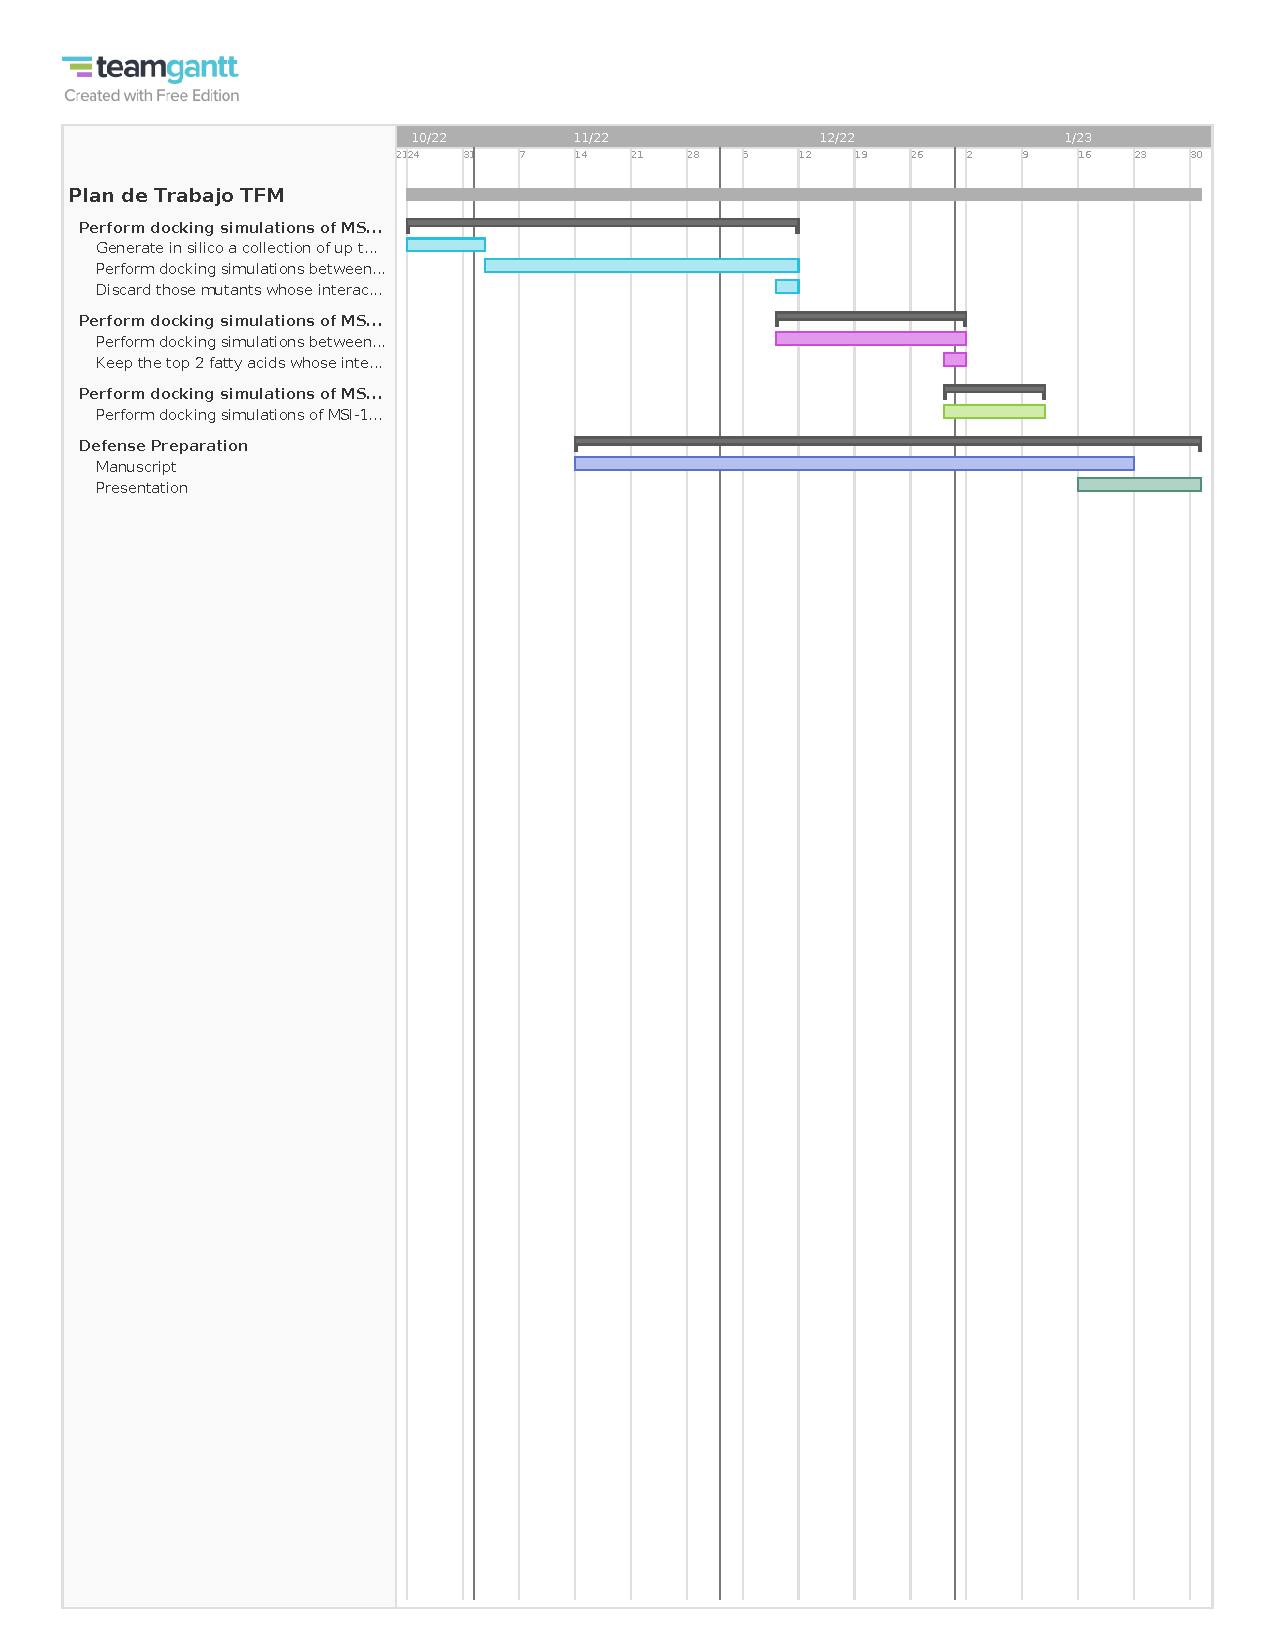
\includegraphics[width=\linewidth, trim={1cm 18.5cm 1cm 2cm},clip]{assets/Plan_de_Trabajo_TFM.pdf}
    \caption{Work plan summarized in a Gnatt chart.}
    \label{fig:gnatt}    
\end{figure}

\subsection{Summary of obtained products}

The main products of this work are:

\begin{enumerate}
    \item The current Master's Thesis manuscript.
    \item 3D structures of 5 MSI-1 RNA-motifs used in \cite{dolcemascolo_2022}.
    \item\textit{los modelos o lo que salga}
    \item\textit{los scripts del pipeline}
    \item\href{https://lightdock.org/tutorials/0.9.3/rna_docking}{A step-by-step tutorial on how to perform a simple protein-RNA docking with \texttt{LightDock}}.
\end{enumerate}

Resulting products are available in different repositories:
\begin{enumerate}
    \item The direct products of this work are present in \href{https://github.com/luksgrin/UOC_TFM}{this \texttt{GitHub} repository}.
    \item The step-by-step tutorial on how to perform a simple protein-RNA docking with \texttt{LightDock} is available at \href{https://github.com/lightdock/lightdock.github.io}{the \texttt{LightDock} \texttt{GitHub} repository}, and on the \href{https://lightdock.org/tutorials/}{\texttt{LightDock} tutorials page}.
\end{enumerate}

\subsection{Summary of other sections of this report}

% Breve explicación de los contenidos de cada capítulo y su relación con el proyecto global. 

The remaing sections of this manuscript are:

\begin{itemize}
    \item\textbf{State of the art}
    \item\textbf{Materials and methods}
    \item\textbf{Results}
    \item\textbf{Conclusions and further work}
    \item\textbf{Glossary}
    \item\textbf{References}
    \item\textbf{Appendix}
\end{itemize}

% \section{Relación de las desviaciones en la temporización y acciones de mitigación si procede y actualización del cronograma si procede}

% Debido a las complicaciones en \texttt{lightdock} a la hora de simular docking del tipo proteína-RNA, y tras consultar esto con el supervisor de este trabajo, se ha decidido desechar la parte de dinámica molecular.\\

% Adicionalmente, este cambio se ha visto reflejado en el título de este trabajo, el cual ha sido modificado de ``\textit{Molecular dynamics of Musashi-1 allosteric RNA-binding sites}'' a ``\textit{Docking assays of Musashi-1 allosteric RNA-binding sites}''. Este cambio ha sido consultado con el supervisor de este trabajo.\\
\pagebreak

% Section 2: State of the art
\section{State of the art}

% Estado del arte del tema en cuestión.
% Debería acabar mostrando por qué el trabajo es importante y aporta algo y con las hipótesis del trabajo.

\subsection{Synthetic Biology}
Synthetic Biology is a modern niche of Biology in which the characteristic ``know-how'' from engineering fields is combined with classical Molecular Biology techniques. Guided by physicist Richard Feynman's famous quote ``\textit{what I cannot create, I do not understand}'', synthetic biologists have developed a deep understanding of how cells control and regulate the processes of gene transcription, translation, metabolite biosynthesis and degradation.\\

It is ``synthetic'' in the sense that synthetic biologists engineer novel (absent in nature) genetic constructions with biological ``pieces'', which usually originate from various different organisms, in order to achieve a phenotype in a target organism that lacks said phenotype in nature. Furthermore, this design usually comes with a mathematical model based in physical first principles of how the system should behave.\\

One of the first successful constructions of this type, and most likely the most popular one, is Gardner's toggle switch \cite{gardner_2000} where they engineered a synthetic toggle switch within \textit{E. coli} by using two different promoters that repressed each other, achieving this way bistability (either one promoter is repressed, or the other). Simultaneously, Elowitz' repressilator \cite{elowitz_2000} was published, where they engineered a synthetic ``clock'' within \textit{E. coli} by chaining 3 repressive promoters that repressed one another in chain, in such a way that the genes controlled by them had periodic expression.\\

These constructions, and all the ones that followed, would not have been possible without a (by then, small) repository of genetic parts, which in turn would not have been possible without the arduous work of an innumerable amount of traditional molecular biologists that sequenced and characterized said parts.In fact, the iGEM foundation keeps a repository of standarized biological parts \cite{parts_igem} along with various data such as the assembly methods used, levels of expression, polymerase used, etc...\\

However, there is still a need for more biological parts, especially parts that are ``orthogonal'', i.e. they can co-exist and function correcly within the same organism without deviating from their theoretical behavior. 

% RNA binding proteins
\subsection{RNA-binding proteins}

% Doking
\subsection{Molecular Docking}
\pagebreak

% Section 3: Materials and methods
\section{Materials and methods}

% En estos capítulos, es necesario describir:
% •	los aspectos más relevantes del diseño y desarrollo del trabajo
% •	la metodología elegida para realizar este desarrollo, describiendo las alternativas posibles, las decisiones tomadas, y los criterios utilizados para tomar estas decisiones.
% •	descripción de los productos obtenidos.
 
% La estructuración de los capítulos puede variar en función del tipo de trabajo.  
 
% En caso de que proceda, se incluirá un apartado de “Valoración económica del trabajo”. Este apartado indicará los gastos asociados al desarrollo y mantenimiento del trabajo, así como los beneficios económicos obtenidos y un análisis final sobre la viabilidad del producto.

\subsection{Data Acquisition}

\subsubsection{Mouse MSI-1 and MSI-1's RMM1}

\href{https://www.uniprot.org/}{\texttt{Uniprot}'s database} was consulted for the structure of the mouse MSI-1 protein (see \textbf{Figure \ref{fig:Q61474uniprot}}). Unfortunately, there was no NMR crystal structure for the complete protein: the only available complete structure was \texttt{AlphaFold}'s prediction of the structure (see \textbf{Figure \ref{fig:3DMSI}}). Said structure had low confidence in the aminoacid sequence not corresponding to the RRMs. Therefore, the crystal structure of MSI-1's RRM1 (see \textbf{Figure \ref{fig:3DRRM1}}) was to be employed instead for the docking simulations.

\begin{figure}[htbp!]
    \centering
    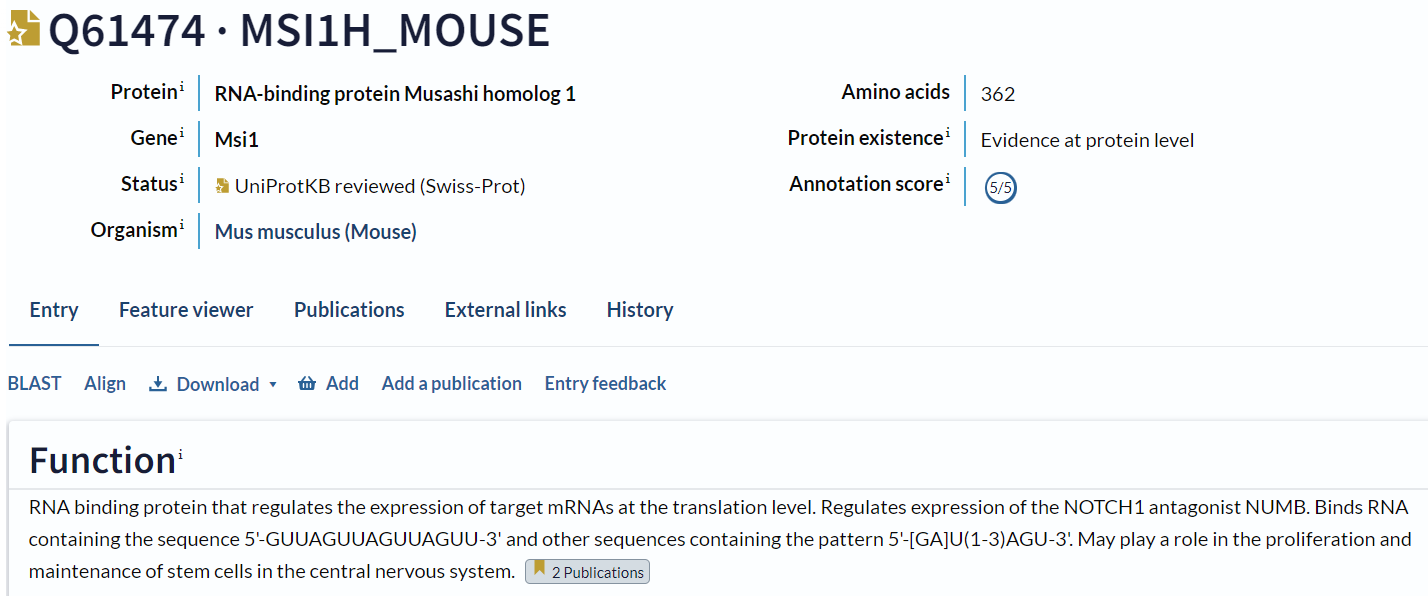
\includegraphics[width=\linewidth]{assets/Q61474_uniprot_entry.png}
    \caption[\href{https://www.uniprot.org/uniprotkb/Q61474/entry}{Uniprot entry Q61474} corresponding to the mouse MSI-1.]{\href{https://www.uniprot.org/uniprotkb/Q61474/entry}{Uniprot entry Q61474} corresponding to the mouse MSI-1 (as seen on 08/01/2023).}
    \label{fig:Q61474uniprot}
\end{figure}

The crystal NMR structure was downloaded as a \texttt{.pdb} file.

\subsubsection{Fatty acids}

The fatty acids to be employed down the line in the docking simulations were retrieved from their respective \href{https://www.chemspider.com/}{\texttt{Chemspider}} entries. The fatty acids downloaded were:

\begin{itemize}
    \item\href{https://www.chemspider.com/Chemical-Structure.392692.html}{arachidonic acid}
    \item\href{https://www.chemspider.com/Chemical-Structure.4444105.html}{linoleic acid}
    \item\href{https://www.chemspider.com/Chemical-Structure.393217.html}{oleic acid}
    \item\href{https://www.chemspider.com/Chemical-Structure.960.html}{palmitic acid}
    \item\href{https://www.chemspider.com/Chemical-Structure.5091.html}{stearic acid}
\end{itemize}

The molecules are shown in \textbf{Figure \ref{fig:fatty_acids}}.

\begin{figure}[htbp!]
    \centering
    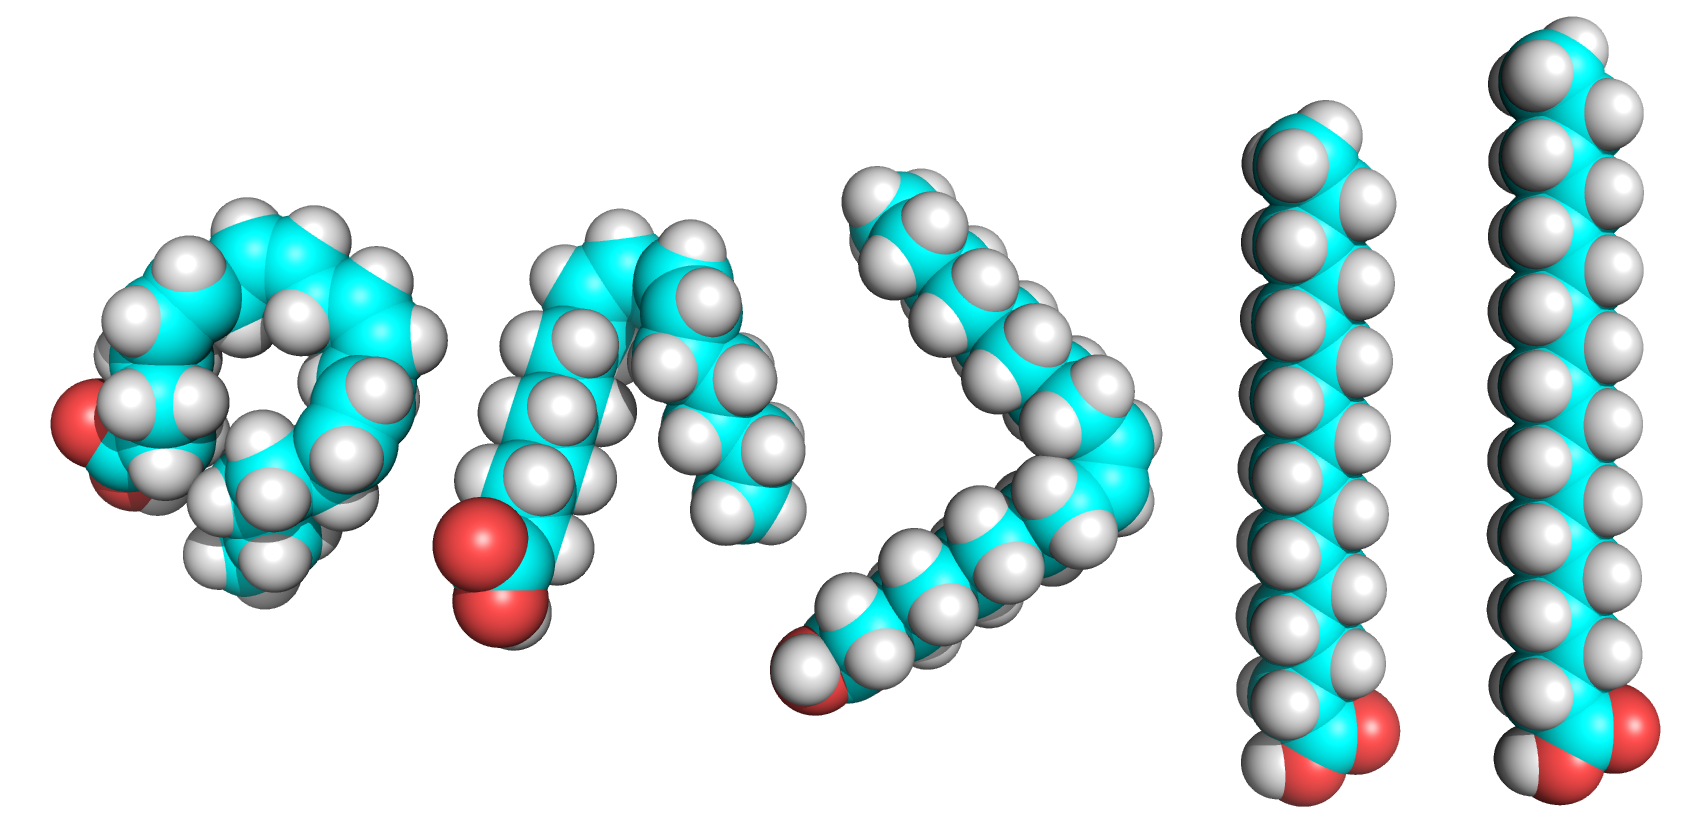
\includegraphics[width=0.75\linewidth]{assets/fatty_acids.png}
    \caption[3D structure of the fatty acids to be employed.]{3D structure of the fatty acids to be employed. From left to right: arachidonic acid, linoleic acid, oleic acid, palmitic acid and stearic acid. Colors represent the atoms present in the structures: cyan is Carbon, red is Oxygen and white is Hydrogen. Visualized through \href{https://pymol.org/2/}{\texttt{Pymol}}.}
    \label{fig:fatty_acids}
\end{figure}

The molecules' 3D structures were downloaded as \texttt{.mol} files. 

\subsection{Generation of 3D RNA molecule structures}

The raw RNA sequences to be employed were retrieved from \cite{dolcemascolo_2022} and are shown in \textbf{\nameref{appendix_A}}, where they crafted small RNA oligos based on a the selex optimal RNA sequence. RNA takes specific spatial conformations when in aqueous media, be it \textit{in vitro} or \textit{in vivo}, which can be computed directly from the RNA sequence by means of pre-measured experimental parameters \cite{santalucia_1998}.\\

To do so, the Nupack software was employed \cite{dirks_2004} (specifically its associated \texttt{Python} package) and the structures in dot-bracket notation\footnote{Dot-bracket notation is a simplistic manner of representing DNA or RNA secondary structure. For more details, see \cite{rna_structure_notations}.} were recorded. In addition, the sequences were subjected to pairwise alignments (by means of MAFFT \cite{katoh_2002}) to highlight the mutations present with respect to the original oligo. The \texttt{Python} script employed to perform these computations is found in \textbf{\nameref{appendix_B}}.

\vfill

\pagebreak

The results are shown in \textbf{Figure \ref{fig:dataset}}:

\begin{figure}[htbp!]
    \lstinputlisting[basicstyle=\tiny]{assets/dataset.tsv}
    \caption{RNA sequences along with the result of the pairwise alingments and Nupack's prediction of their secondary structure.}
    \label{fig:dataset}
\end{figure}

With this information (RNA sequence and secondary structure), the 3D conformation of each of the RNA motifs was computed by means of the \href{https://rnacomposer.cs.put.poznan.pl/}{\texttt{RNAComposer}} web server \cite{biesiada_2016} and downloaded in \texttt{.pdb} format. The corresponding 3D structures of the RNA motifs are shown in \textbf{Figure \ref{fig:RNAs}}.

\begin{figure}[htbp!]
    \centering
    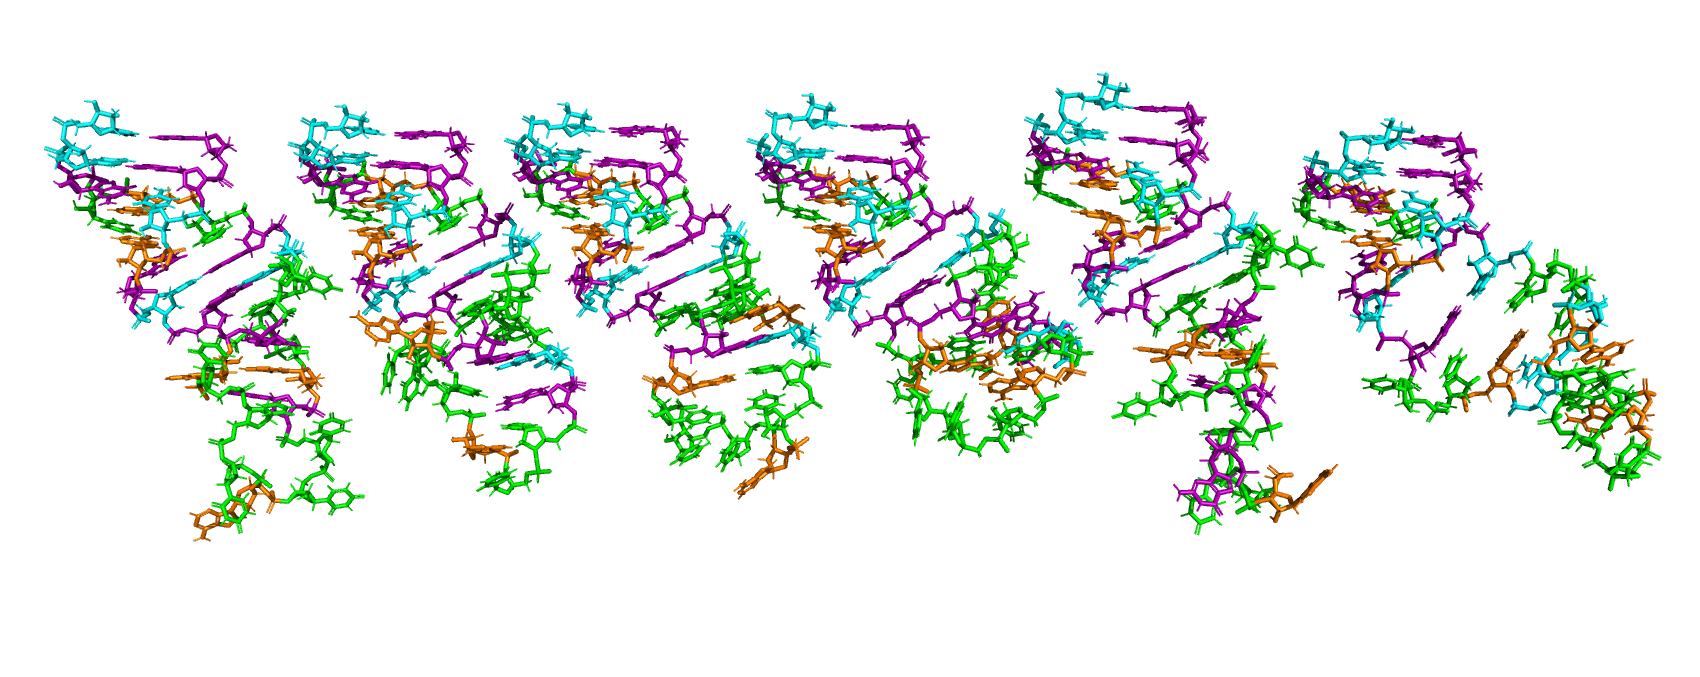
\includegraphics[width=\linewidth]{assets/RNAs.png}
    \caption[3D structures of the RNA motifs.]{3D structures of the RNA motifs. From left to right: the original RNA motif followed by the 5 mutants. Colors represent the nucleotidic bases: orange is Adenine, purple is Guanine, cyan is Cytosine and green is Uracil. Visualized through \href{https://pymol.org/2/}{\texttt{Pymol}}.}
    \label{fig:RNAs}
\end{figure}

With the 3D structures of the RNA motifs, the next step is to prepare the protein-RNA docking simulations.

\subsection{Protein-RNA docking simulations with \texttt{LightDock}}

For the protein-RNA docking simulations, the \texttt{LightDock} \cite{jimenez_garcia_2017} docking software was chosen. The main reasons are the simplicity of \texttt{LightDock}, the quality of the documentation and that the software is written in \texttt{Python}, which eases debugging steps in case of complications. Originally, \texttt{LightDock} was not meant for protein-RNA docking simulations. However, by means of some reasearch and auxiliary \texttt{Python} scripts, a simple and novel pipeline was designed which makes it possible to perform such docking simulations with \texttt{LightDock}. This pipeline takes inspiration on the \href{https://lightdock.org/tutorials/0.9.3/dna_docking}{protein-DNA docking example tutorial from the \texttt{LightDock} documentation}.

\subsubsection{Protein preparation}

First, MSI-1's RRM1 \texttt{.pdb} file needs to have their hydrogen atoms modified and relabeled so that they match the \texttt{AMBER94} force field, which is the parameter set that is going to be used in this docking simulation. To do so, the softwares \href{https://github.com/rlabduke/reduce}{\texttt{REDUCE}} and \href{https://github.com/haddocking/pdb-tools/}{\texttt{PDB-Tools}} \cite{rodrigues_2018} were employed.\\

In addition, the MSI-1's RRM1 \texttt{.pdb} file needed an additional motification related to the \texttt{AMBER94} force field: regular \texttt{.pdb} files employ the \texttt{HIS} identifier for the histidine aminoacid, which does not appear in the \texttt{AMBER94} force field. The reason behind this is that for the \texttt{AMBER94} force field, histidine can be one of 3 possible residues \cite{amber_histidine}:

\begin{enumerate}
    \item\texttt{HID}: histidine with a single hydrogen on the delta nitrogen
    \item\texttt{HIE}: histidine with a single hydrogen on the epsilon nitrogen
    \item\texttt{HIP}: histidine with hydrogens on both nitrogens (delta and epsilon). This histidine has a positive charge
\end{enumerate}

Therefore, one has to check which kind of histidine residue is present in the molecule, and change it for the corresponding \texttt{AMBER94}-compatible identifier. This can be done with a simple \texttt{Python} script called \texttt{fixHIS}, which is found in \textbf{\nameref{appendix_C}}.

\subsubsection{RNA preparation}

Similar to the protein, the RNA structures' \texttt{.pdb} file need to have their hydrogen atoms modified and relabeled. Again, the softwares \href{https://github.com/rlabduke/reduce}{\texttt{REDUCE}} and \href{https://github.com/haddocking/pdb-tools/}{\texttt{PDB-Tools}} \cite{rodrigues_2018} were employed.\\

In addition, \texttt{REDUCE} adds the 3' and 5' hydroxile groups to the RNA structures. These atoms aren't present in the \texttt{AMBER94} force field, therefore it is mandatory to remove them in order to avoid issues downstream. This can be done with a simple \texttt{Python} script called \texttt{removeEnds.py}, which is found in \textbf{\nameref{appendix_D}}.\\

Next, due to particularities of \texttt{REDUCE} for nucleic acids, it is necessary to rename and remove incompatible atom types present in the RNA structure. Again, this can be done with a simple \texttt{Python} script called \texttt{reduce\_to\_amber.py}, which is found in \textbf{\nameref{appendix_E}}. Note that the aforementioned \texttt{Python} script is an adaptation of the original version provided in the \href{https://lightdock.org/tutorials/0.9.3/dna_docking}{protein-DNA docking example tutorial from the \texttt{LightDock} documentation}.\\

Finally, in order to sucessfully run \texttt{LightDock}'s setup phase, it is mandatory to remove the \texttt{R} tags within the RNA structures. The \texttt{R} tags are important because they indicate which \texttt{AMBER94} parameters to use during the docking simulations, however one of \texttt{LightDock}'s dependencies in the setup phase (\href{http://prody.csb.pitt.edu/}{\texttt{ProDy}}) has conflicts with this notation. This removal can be done with a simple \texttt{Python} script called \texttt{manipulateRNA.py}, which is found in \textbf{\nameref{appendix_F}}.

\subsubsection{\texttt{LightDock} setup and simulation}

\texttt{LightDock}'s setup itself is simple, as it only consists of executing the setup script with the structures prepared in the previous steps, as shown in \textbf{Figure \ref{fig:lightdocksetup}}:

\begin{figure}[htbp!]
    \lstinputlisting[language=bash]{assets/lightdocksetup.sh}
    \caption{\texttt{LightDock} setup command.}
    \label{fig:lightdocksetup}
\end{figure}

The setup will generate, among other files, the simulation-ready structures\linebreak \texttt{lightdock\_protein.pdb} and \texttt{lightdock\_rna.pdb}. For the docking simulation to be successful, it is crucial to add the \texttt{R} tags within the \texttt{lightdock\_rna.pdb} RNA structure, which is basically reversing the tag removal process performed earlier. This can be achieved with a simple \texttt{Python} script called \texttt{manipulateRNAagain.py}, which is found in \textbf{\nameref{appendix_G}}.\\

\subsubsection{\texttt{LightDock} docking simulation, clustering and ranking}

If the previous steps executed without issues, it is possible to run \texttt{LightDock} as shown in \texttt{Figure \ref{fig:lightdockexec}}:

\begin{figure}[htbp!]
    \lstinputlisting[language=bash]{assets/lightdockexec.sh}
    \caption[\texttt{LightDock} execution command.]{\texttt{LightDock} execution command, using the \texttt{DNA} scoring function for nucleic acids and 4 processing cores.}
    \label{fig:lightdockexec}
\end{figure}

Once the simulation ends, and in order to be able to do the clustering and ranking step, it is mandatory to remove the \texttt{R} tags added to \texttt{lightdock\_rna.pdb} for the simulation step. For that, once again the script \texttt{manipulateRNA.py} shown in \textbf{\nameref{appendix_F}} is employed.\\

Next, the clustering and ranking can be performed in the same way as specified in the \href{https://lightdock.org/tutorials/0.9.3/dna_docking}{protein-DNA docking example tutorial from the \texttt{LightDock} documentation}. The \texttt{bash} script performing the ranking and clustering steps is shown in \textbf{\nameref{appendix_H}}.\\

The ranking will generate a \texttt{solutions.list} file where the different models generated by \texttt{LightDock} are scored. For this work, the top 10 best scoring models were taken.\\

The entire pipeline followed in this section has been implemented as a \texttt{bash} script called \texttt{run1.sh}, which is found in \textbf{\nameref{appendix_I}}. Given a\linebreak\texttt{target\_protein.pdb} file and a \texttt{ligand\_rna.pdb} file, \texttt{run1.sh} is executed as shown in \textbf{Figure \ref{fig:execrun1}}:

\begin{figure}[htbp!]
    \lstinputlisting[language=bash]{assets/run1exec.sh}
    \caption[Execution of the \texttt{run1.sh} script.]{Execution of the \texttt{run1.sh} script.}
    \label{fig:execrun1}
\end{figure}

A refined version of this pipeline has been contributed to the \href{https://lightdock.org/tutorials/0.9.3/index.html}{official \texttt{LightDock} tutorials section}. In said version, the \texttt{Python} scripts for file manipulation have been cleaned-up and applied to model the \href{https://www.rcsb.org/structure/1a1t}{1A1T protein-RNA complex}. This tutorial can be directly accessed \href{https://lightdock.org/tutorials/0.9.3/rna_docking}{here}.

% Las siguientes subsecciones son la liada parda que aún he de arreglar
\subsection{Fatty acid-protein docking simulations}
\subsection{Fatty acid-protein-RNA docking simulations}

\pagebreak

% Section 4: Results
\section{Results}

% Detallad en este apartado los resultados obtenidos utilizando la metodología descrita en el apartado anterior.
\pagebreak

% Section 5: Conclusions and further work
\section{Conclusions and further work}

The main objective of this Master's Thesis was to extend the knowledge behind of the allosteric interactions occurring in the MSI-1 proteins.\\

% •	Una descripción de las conclusiones del trabajo:
% ¿Una vez se han obtenido los resultados qué conclusiones se extrae?
From the results observed, it can be concluded that the allosteric behavior of MSI-1 must stem from a conformational change deep within the protein, triggered by the non-polar nature of the fatty acid's hydrocarbon chain, consequently altering the RNA binding region. The efficiency at which a particular fatty acid induces said conformational change is yet to be studied.\\

However, the lipid-RRM1 models hint that the smaller and more flexible the fatty acid molecule is, the more capability it may have to induce conformational changes as it can explore RRM1's fatty acid binding ``pocket'' in more depth. As a consequence, the fatty acid interacts with a larger amount of aminoacids, changing their chemical environment and forcing a rearrangement that can spread to the RNA binding site.\\

% ¿Estos resultados son los esperados? ¿O han sido sorprendentes? ¿Por qué?
The results obtained were partially expected: allosteric proteins undergo conformational changes when bound to their different ligands. However, it was also expected to obtain successful models for each of the RNA motif mutants to understand the effect of the RNA nucleic acid sequence itself on the interaction. Unfortunately, due to the unsatisfactory models obtained, this question will remain unanswered in this work.\\

% •	Una reflexión crítica sobre la consecución de los objetivos planteados inicialmente:
% ¿Hemos alcanzado todos los objetivos? Si la respuesta es negativa, ¿por qué?
% •	Un análisis crítico del seguimiento de la planificación y metodología a lo largo del producto:
% -	¿Se ha seguido la planificación?
% -	¿La metodología prevista ha sido suficientemente adecuada?
% -	¿Ha sido necesario introducir cambios para garantizar el éxito del trabajo? ¿Por qué?
The objectives stated during the initial phases of this work differ vastly from the objectives stated and accomplished in this report. Originally, each docking simulation would have been chaperoned by molecular dynamics simulations, which would have shed additional light on the matter of the allosteric behavior of RRM1. These molecular dynamics simulations were eventually scraped out from the objectives due to lack of time caused by solving troubles in the protein-RNA docking step.\\

Nonetheless, solving those problems resulted in a collaboration with the\linebreak\texttt{LightDock} team for a public tutorial on how to use \texttt{LightDock} for protein-RNA docking, so it was worth the time.\\

% •	Las líneas de trabajo futuro que no han podido explorarse en este trabajo y han quedado pendientes.
Therefore, additional further work could be focused on molecular dynamics assays of the allosteric interactions in MSI-1, as there is expected to observe interesting conformational changes when the ligands approach and bind RRM1.\\

It would also be of interest to assess the strength of the protein-RNA interaction in such a way that it made possible the intelligent design of RNA ligands with pre-computed affinity.\\

Additionally, it would be of great benefit for the general public to extend\linebreak\texttt{LightDock}'s functionalities into lipid-protein docking, or even general small\linebreak molecule-protein docking.\\

In sum, docking simulations have a great potential of untangling molecular mysteries such as the one involving MSI-1's allosteric nature. Nonetheless, there are still some limitations as the resulting models are not always reliable. So, there is much work to do to improve the exciting field of structural bioinformatics. Again, as Richard Feynman once said: ``\textit{what I cannot create, I do not understand}''.
\pagebreak

% Section 6: Glossary
\section{Glossary}
% Definición de los términos y acrónimos más relevantes utilizados en la Memoria.

\begin{itemize}
    \item[]\textbf{MSI-1}: Neural Musashi-1 protein.
    \item[]\textbf{RBP}: RNA-binding protein.
    \item[]\textbf{RRM}: RNA recognition motif
    \item[]\textbf{NMR}: Nuclear magnetic resonance.
    \item[]\textbf\textit{E. coli}: \textit{Escherichia coli}.
    \item[]\textbf{iGEM}: International genetically engineered machine competition.
    \item[]\textbf{RNA}: Ribonucleic acid.
    \item[]\textbf{RNA}: Deoxyribonucleic acid.
    \item[]\textbf{LUCA}: Last universal common ancestor.
    \item[]\texttt{.pdb}: Protein data bank file extension.
    \item[]\texttt{.mol}: MDL Molfile format file extension.
    \item[]\texttt{.fasta}: FASTA format file extension.
    \item[]\texttt{MAFFT}: Multiple alignment using fast Fourier transform algorithm.
\end{itemize}
\pagebreak

% Section 7: References
\bibliographystyle{ieeetr}
\bibliography{references.bib}
% Lista numerada de las referencias bibliográficas utilizadas en la memoria. En cada lugar donde se utilice una referencia dentro del texto, debe indicarse citando el número de la referencia, por ejemplo: [7].
 
% Es muy importante incluir todas las referencias utilizadas y citarlas apropiadamente, es decir, incluyendo toda la información necesaria para identificar la referencia. La información mínima a incluir según el tipo de referencia es:
 
% •	Libro: Autores, Título, Edición (en su caso) Editorial, Ciudad, Año.
% •	Artículo de revista: Autores, Título, Nombre de la Revista, Número de Página inicial y final, Número de la revista / Volumen, Año.
% •	Web: URL y fecha en la que se ha visitado.	

\pagebreak

% Section 8: Appendix
\setcounter{page}{1}
\pagenumbering{Roman}

\section{Appendix}

% Listado de apartados que son demasiado extensos para incluir en la memoria y tienen un carácter autocontenido (por ejemplo, manuales de usuario, manuales de instalación, etc.)
 
% Dependiendo del tipo de trabajo, es posible que no sea necesario añadir ningún anexo.



% \subsection*{Anexo A: Motivos de RNA empleados en este trabajo (en formato \texttt{.fasta})}\label{anexo_A}
% \addcontentsline{toc}{subsection}{Anexo A: Motivos de RNA empleados en este trabajo (en formato \texttt{.fasta})}

% \lstinputlisting{assets/motifs.fasta}

% \subsection*{Anexo B: Motivos de RNA junto a su alineamiento con la secuencia original y estructura secundaria}\label{anexo_B}
% \addcontentsline{toc}{subsection}{Anexo B: Motivos de RNA junto a su alineamiento con la secuencia original y estructura secundaria}

% \lstinputlisting[basicstyle=\tiny]{assets/dataset.tsv}

% \subsection*{Anexo C: Script de \texttt{Python} para el tratamiento de los motivos de RNA}\label{anexo_C}
% \addcontentsline{toc}{subsection}{Anexo C: Script de \texttt{Python} para el tratamiento de los motivos de RNA}

% \lstinputlisting[language=Python]{assets/motifs_treatment.py}

% \subsection*{Anexo D: Conformaciones 3D de los motivos de RNA}\label{anexo_D}
% \addcontentsline{toc}{subsection}{Anexo D: Conformaciones 3D de los motivos de RNA}

% \begin{center}
%     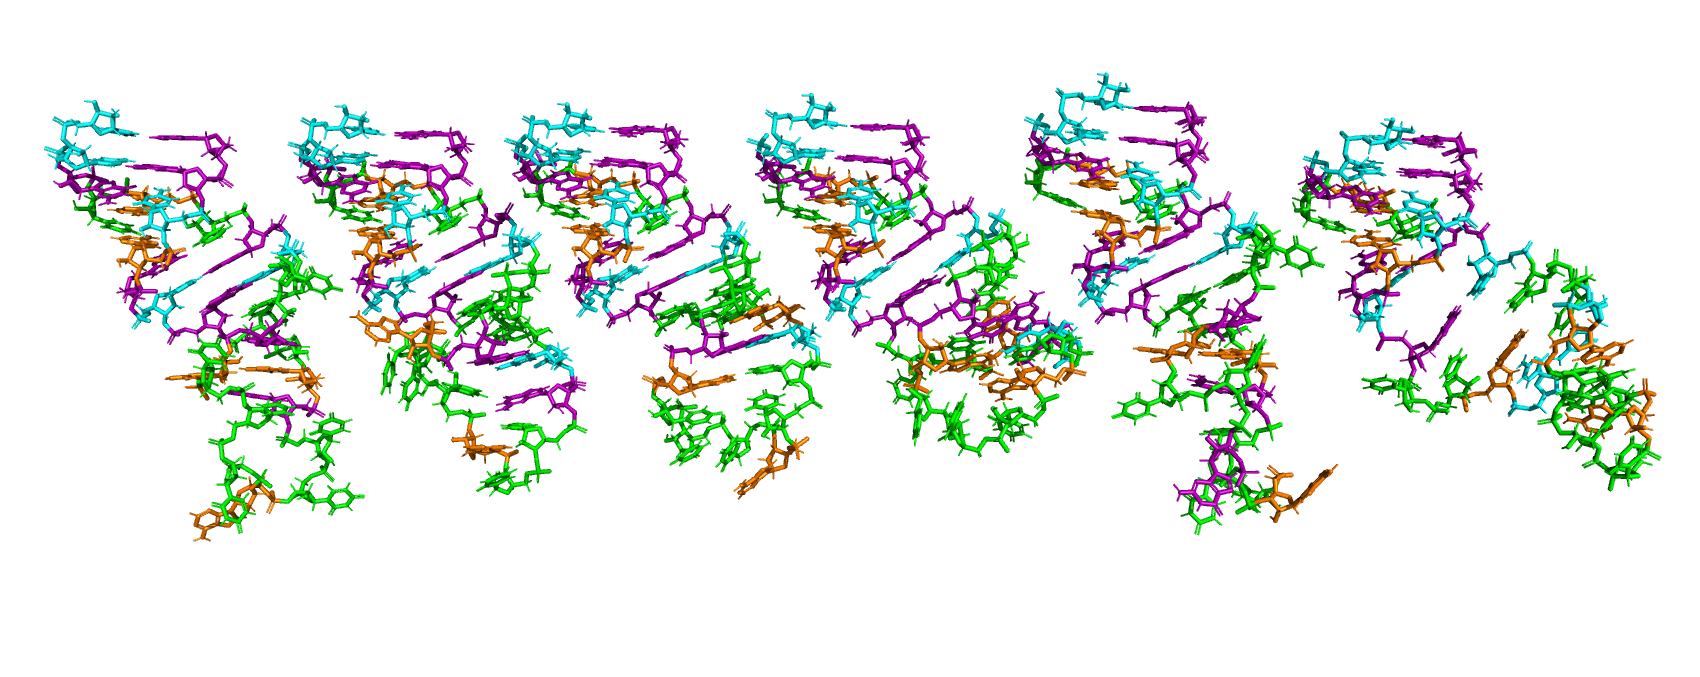
\includegraphics[width=\linewidth]{assets/RNAs.png}
% \end{center}

% De izquierda a derecha: el motivo de RNA original seguido de los 5 mutantes. Los colores representan las bases nucleotídicas: naranja es Adenina, violeta es Guanina, cian es Citosina y verde es Uracilo. Visualizado con \href{https://pymol.org/2/}{\texttt{Pymol}}.

% \subsection*{Anexo G: Visualización de la estructura 3D de los ácidos grasos}\label{anexo_G}
% \addcontentsline{toc}{subsection}{Anexo G: Visualización de la estructura 3D de los ácidos grasos}

% \begin{center}
%     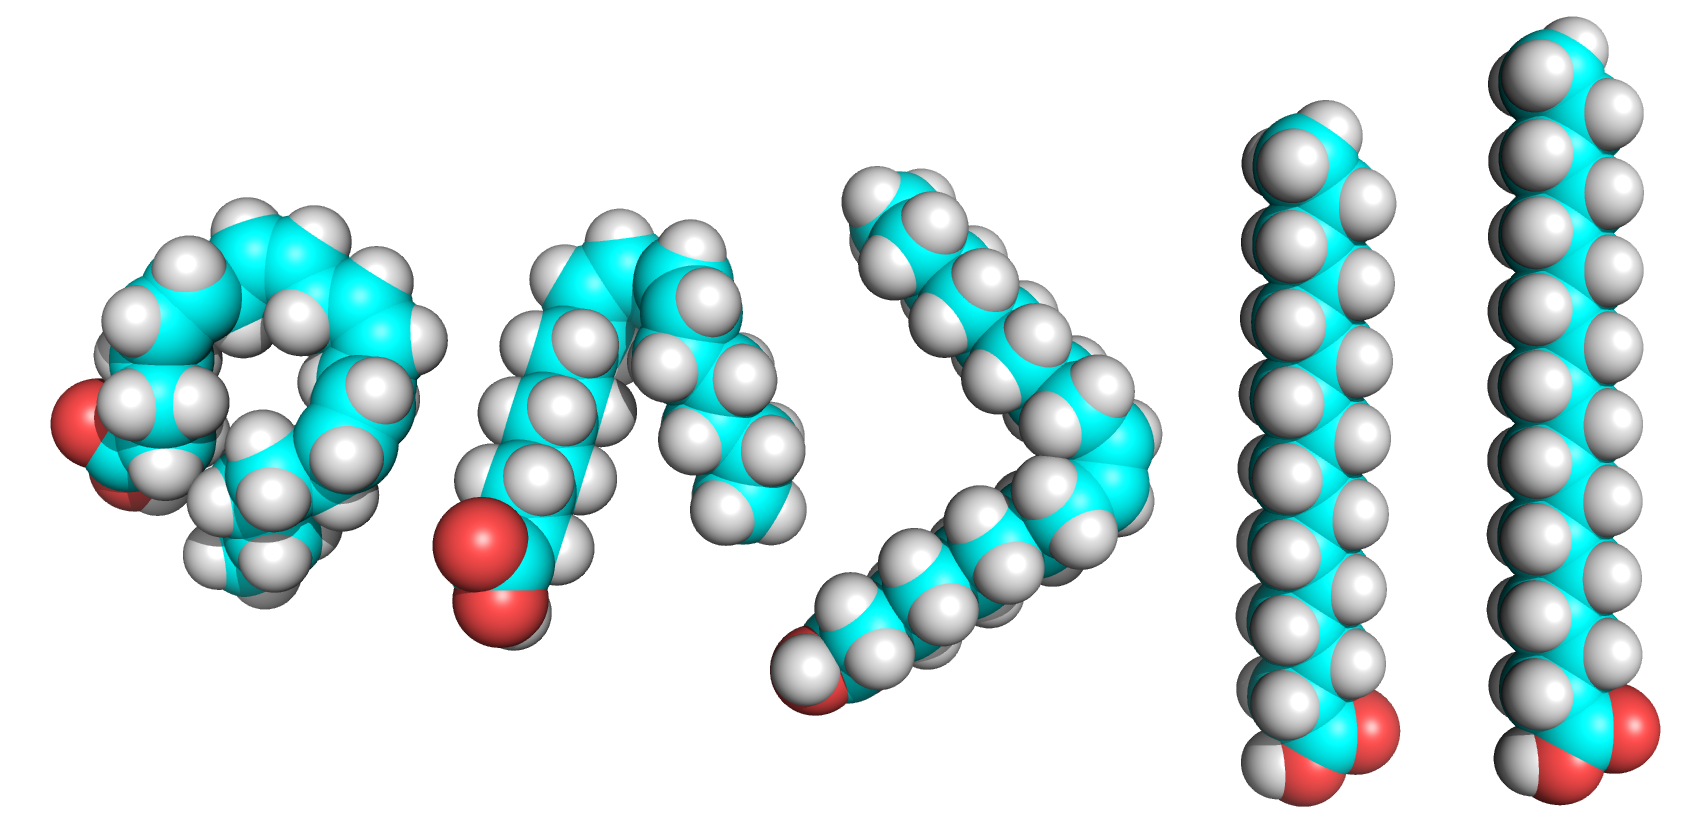
\includegraphics[width=0.633\linewidth]{assets/fatty_acids.png}
% \end{center}

% Visualización en 3D de los ácidos grasos seleccionados. De izquierda a derecha: ácido araquidónico, ácido linoleico, ácido oleico, ácido palmítico y ácido esteárico. Los colores representan los átomos: cian es Carbono, rojo es Oxígeno y blanco es Hidrógeno. Visualizado con \href{https://pymol.org/2/}{\texttt{Pymol}}.

% \subsection*{Anexo A: Script de \texttt{Python} para la mitigación de los tags \texttt{R} en los ficheros \texttt{.pdb} de los RNAs}\label{anexo_A}
% \addcontentsline{toc}{subsection}{Anexo A: Script de \texttt{Python} para la mitigación de los tags \texttt{R} en los ficheros \texttt{.pdb} de los RNAs}

% \lstinputlisting[language=Python]{assets/manipulateRNA.py}

% \subsection*{Anexo B: Script de \texttt{Python} para la recuperación de los tags \texttt{R} en los ficheros \texttt{.pdb} de los RNAs}\label{anexo_B}
% \addcontentsline{toc}{subsection}{Anexo B: Script de \texttt{Python} para la recuperación de los tags \texttt{R} en los ficheros \texttt{.pdb} de los RNAs}

% \lstinputlisting[language=Python]{assets/manipulateRNAagain.py}

% \subsection*{Anexo C: Script de \texttt{Python} para eliminar grupos hydroxilos en los extremos 3' y 5'}\label{anexo_C}
% \addcontentsline{toc}{subsection}{Anexo C: Script de \texttt{Python} para eliminar grupos hydroxilos en los extremos 3' y 5'}

% \lstinputlisting[language=Python]{assets/removeEnds.py}

% \subsection*{Anexo D: Script de \texttt{Python} para re-etiquetar correctamente los resíduos de Histidina}\label{anexo_D}
% \addcontentsline{toc}{subsection}{Anexo D: Script de \texttt{Python} para re-etiquetar correctamente los resíduos de Histidina}

% \lstinputlisting[language=Python]{assets/fixHIS.py}

% \subsection*{Anexo E: Visualización de los 10 mejores modelos de docking entre MSI-1 y el RNA original (\textit{wild type})}\label{anexo_E}
% \addcontentsline{toc}{subsection}{Anexo E: Visualización de los 10 mejores modelos de docking entre MSI-1 y el RNA original (\textit{wild type})}

% \begin{center}
%     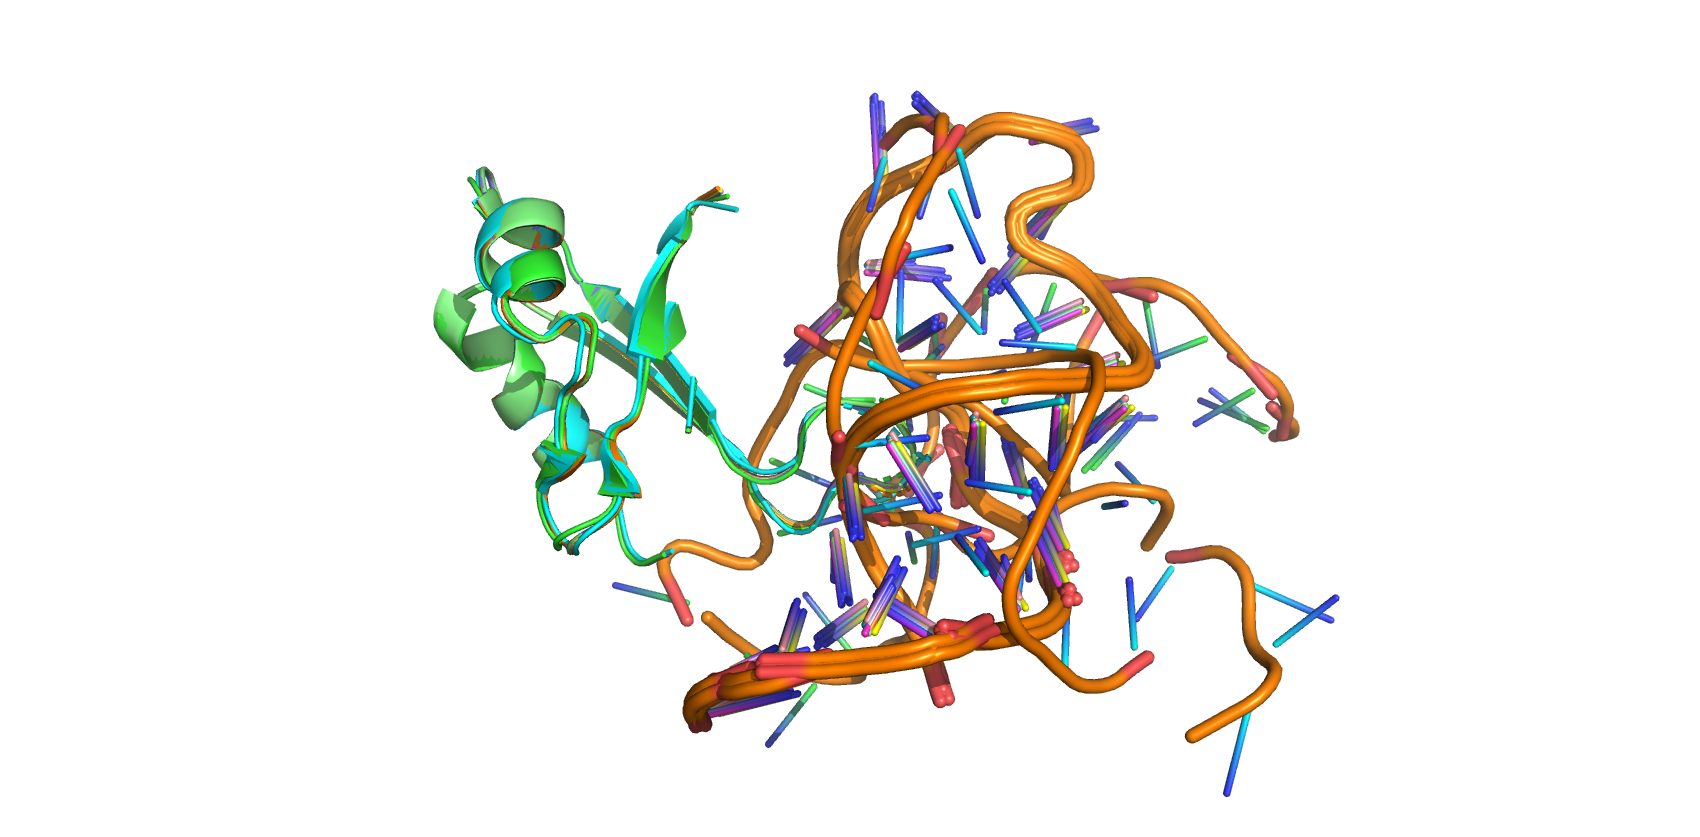
\includegraphics[width=\linewidth]{assets/RMM1_orig_ALL.png}
% \end{center}

% Podemos observar que los modelos difieren entre sí. En los subsiguientes anexos, estos modelos serán desglosados. Visualizado con \href{https://pymol.org/2/}{\texttt{Pymol}}.

% \subsection*{Anexo F: Visualización del mejor modelo de docking entre MSI-1 y el RNA original (\textit{wild type})}\label{anexo_F}
% \addcontentsline{toc}{subsection}{Anexo F: Visualización del mejor modelo de docking entre MSI-1 y el RNA original (\textit{wild type})}

% \begin{center}
%     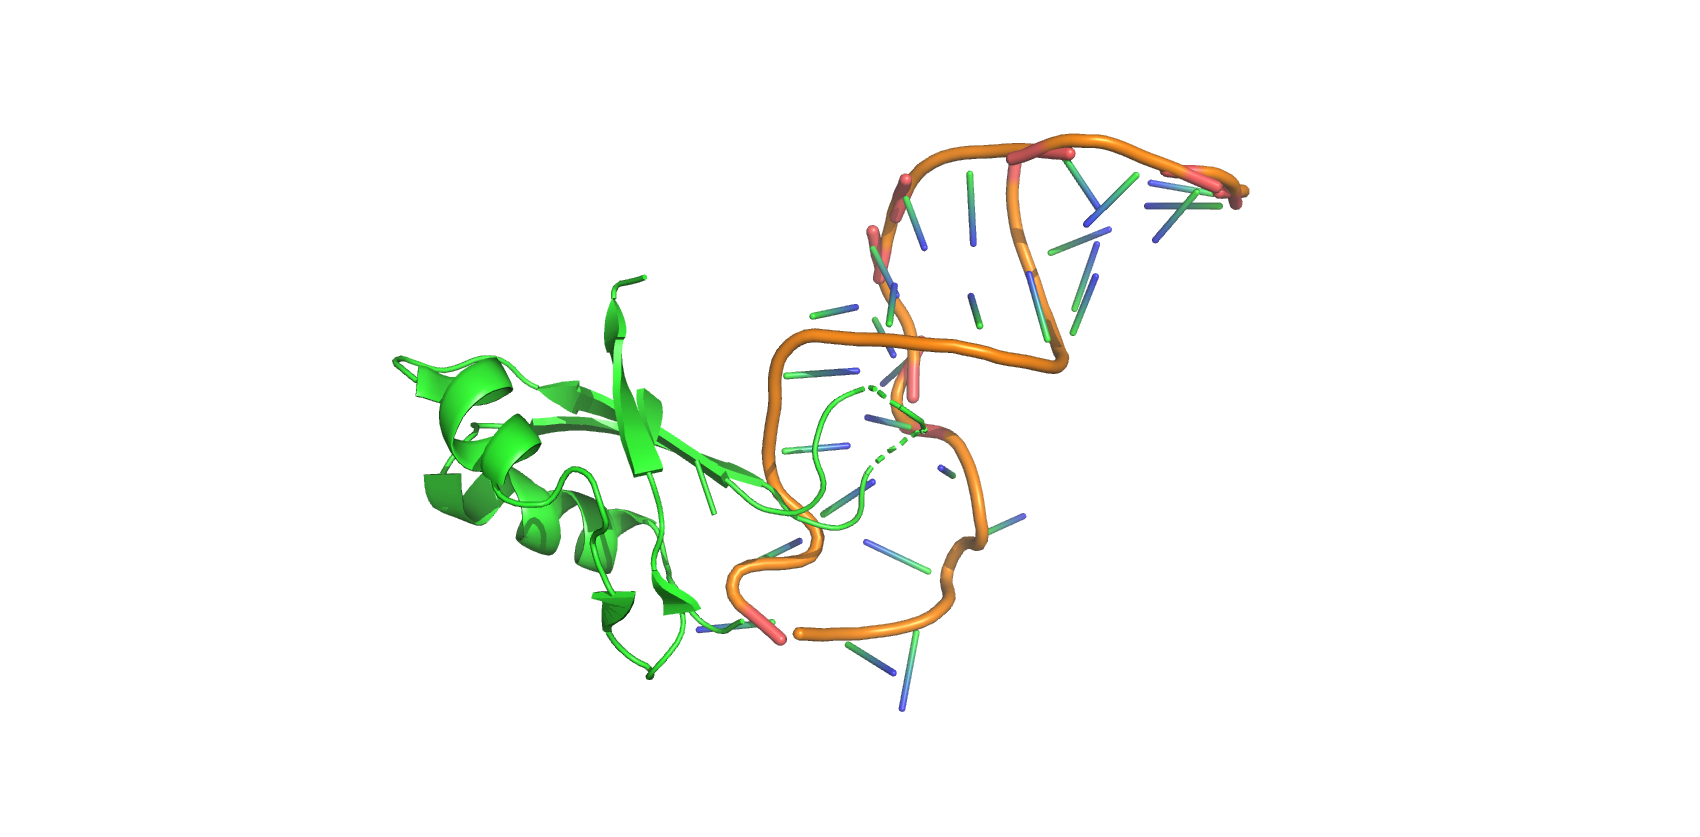
\includegraphics[width=\linewidth]{assets/RMM1_orig_top0.png}
% \end{center}

% Visualizado con \href{https://pymol.org/2/}{\texttt{Pymol}}.

% \subsection*{Anexo G: Visualización del segundo mejor modelo de docking entre MSI-1 y el RNA original (\textit{wild type})}\label{anexo_G}
% \addcontentsline{toc}{subsection}{Anexo G: Visualización del segundo mejor modelo de docking entre MSI-1 y el RNA original (\textit{wild type})}

% \begin{center}
%     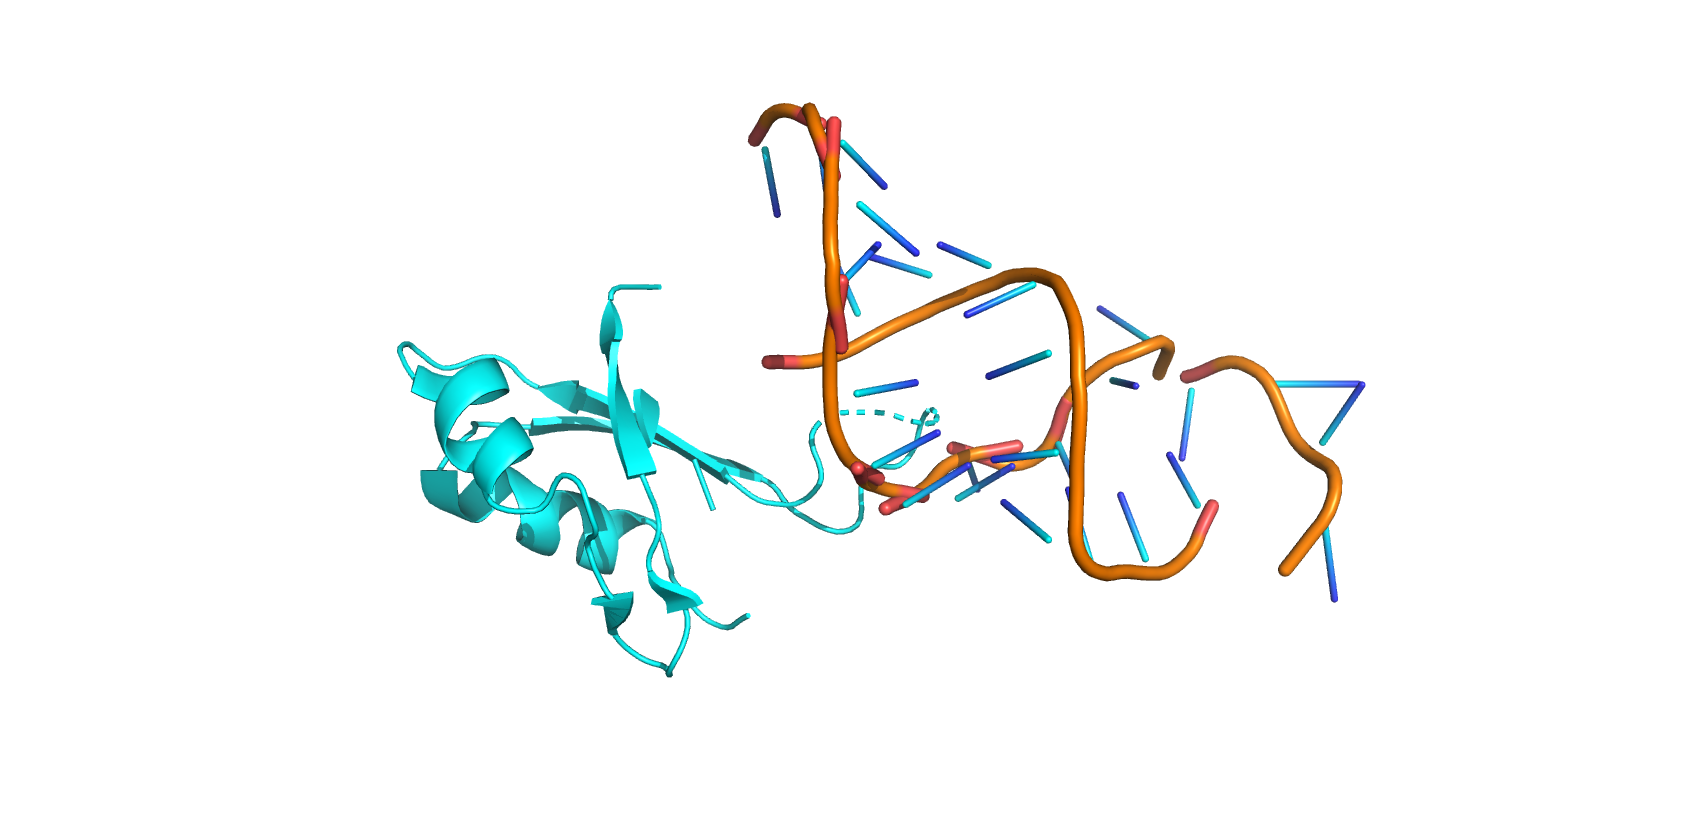
\includegraphics[width=\linewidth]{assets/RMM1_orig_top1.png}
% \end{center}

% Visualizado con \href{https://pymol.org/2/}{\texttt{Pymol}}.

% \subsection*{Anexo H: Visualización del tercer al décimo mejores modelos de docking entre MSI-1 y el RNA original (\textit{wild type})}\label{anexo_H}
% \addcontentsline{toc}{subsection}{Anexo H: Visualización del tercer al décimo mejores modelos de docking entre MSI-1 y el RNA original (\textit{wild type})}

% \begin{center}
%     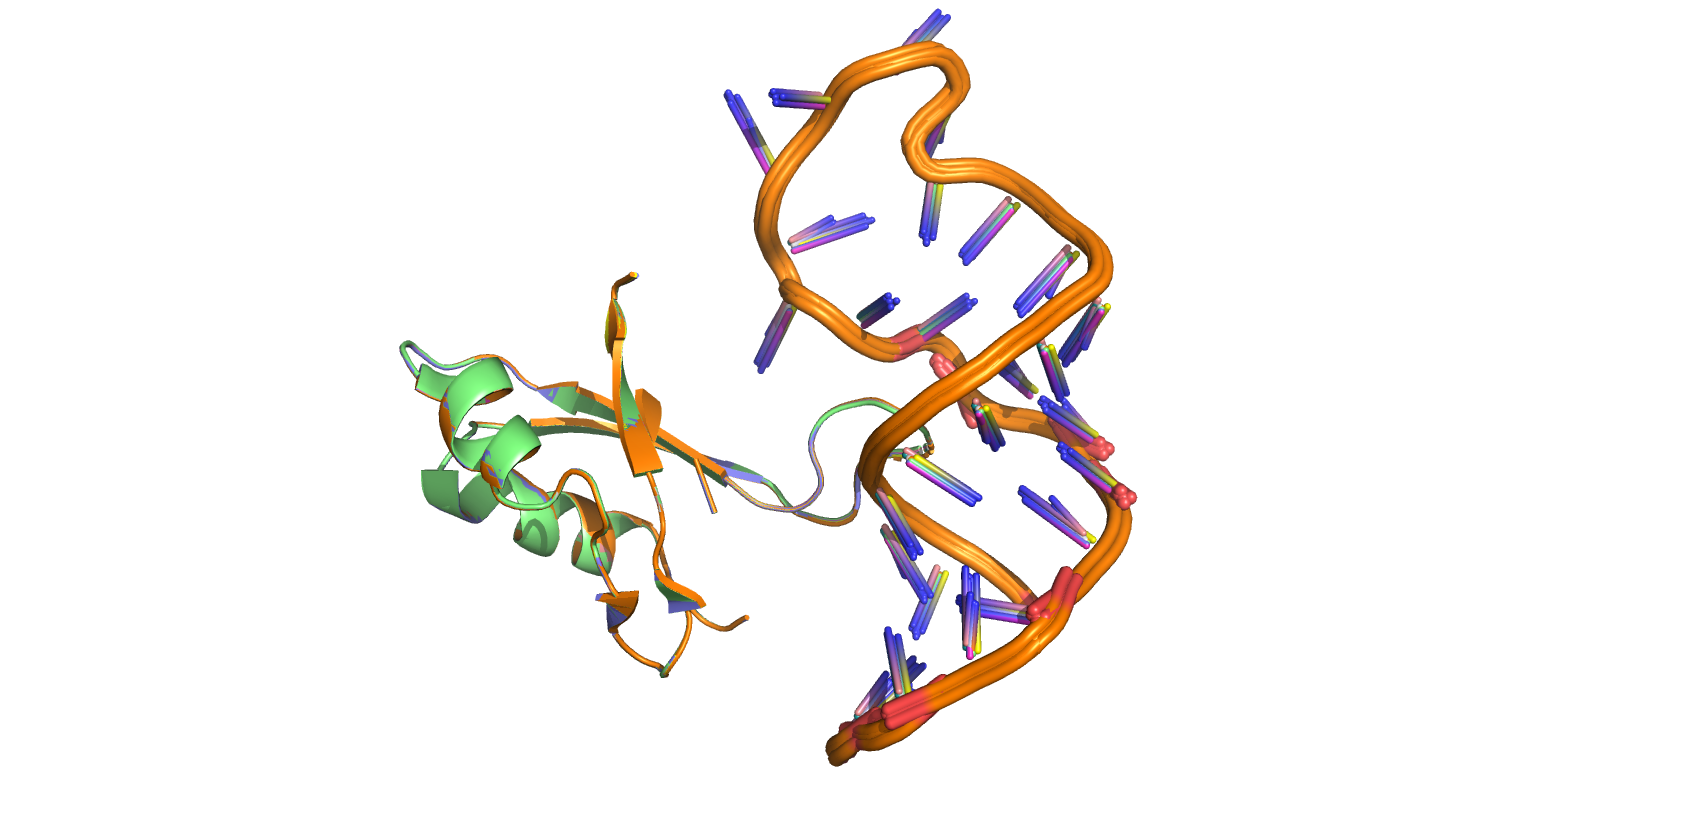
\includegraphics[width=\linewidth]{assets/RMM1_orig_2to8.png}
% \end{center}

% Podemos observar que estos modelos son casi equivalentes. Visualizado con \href{https://pymol.org/2/}{\texttt{Pymol}}.

% \subsection*{Anexo I: Visualización de los 10 mejores modelos de docking entre MSI-1 y el RNA mutante 1}\label{anexo_I}
% \addcontentsline{toc}{subsection}{Anexo I: Visualización de los 10 mejores modelos de docking entre MSI-1 y el RNA mutante 1}

% \begin{center}
%     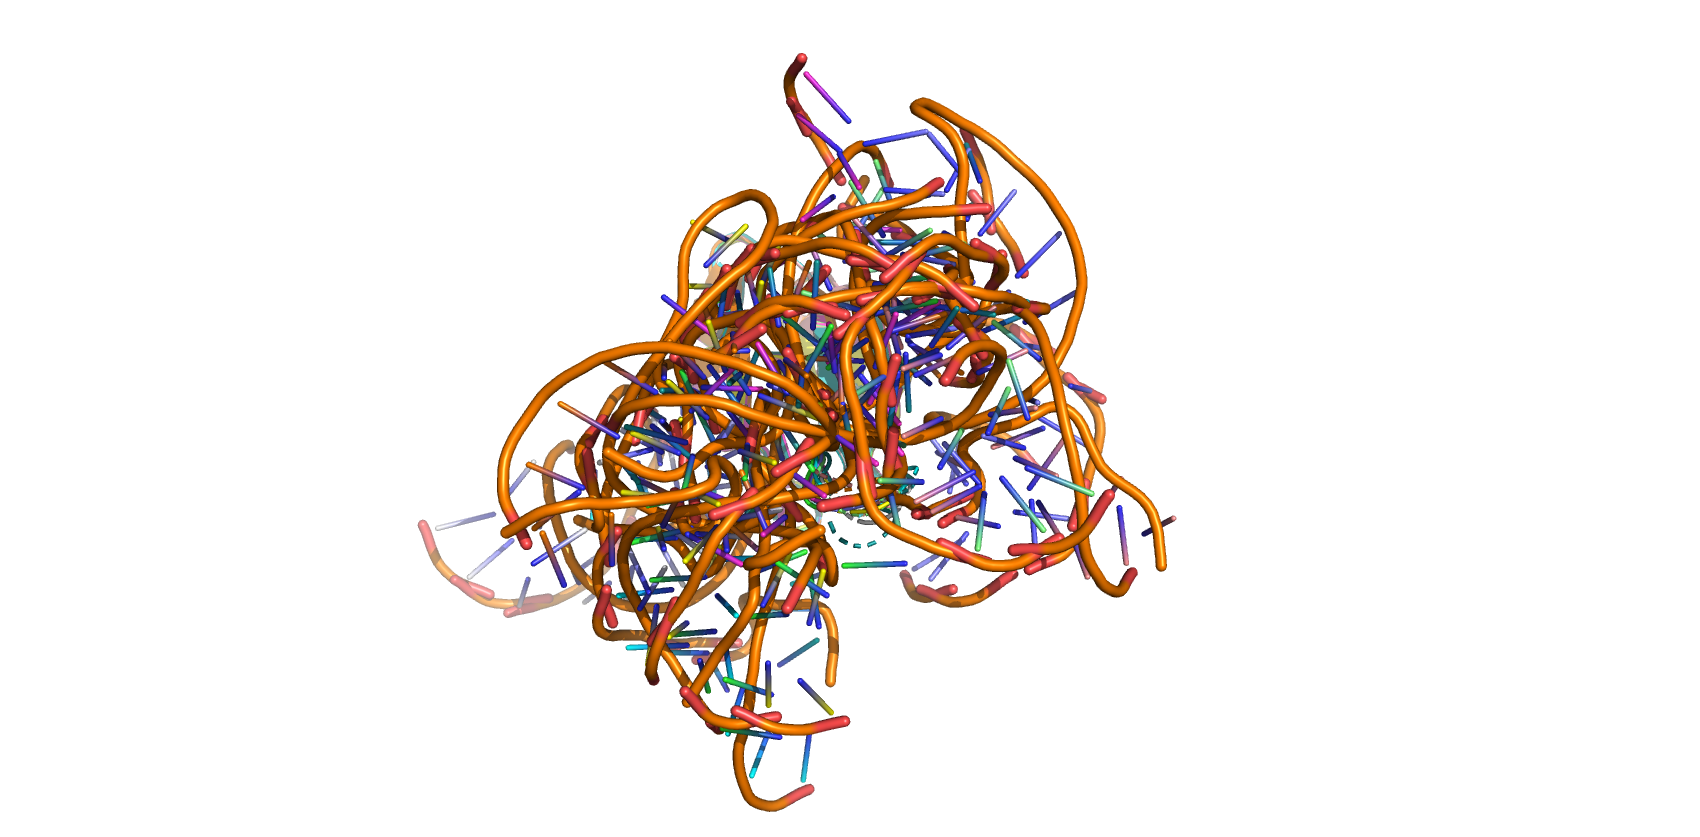
\includegraphics[width=0.9\linewidth]{assets/RMM1_mut1_ALL.png}
% \end{center}

% Podemos observar que los modelos difieren muchísimo entre sí. Parece ser que la mutación desestabiliza la interacción.  Visualizado con \href{https://pymol.org/2/}{\texttt{Pymol}}.

% \subsection*{Anexo J: Visualización de los 10 mejores modelos de docking entre MSI-1 y el RNA mutante 2}\label{anexo_J}
% \addcontentsline{toc}{subsection}{Anexo J: Visualización de los 10 mejores modelos de docking entre MSI-1 y el RNA mutante 2}

% \begin{center}
%     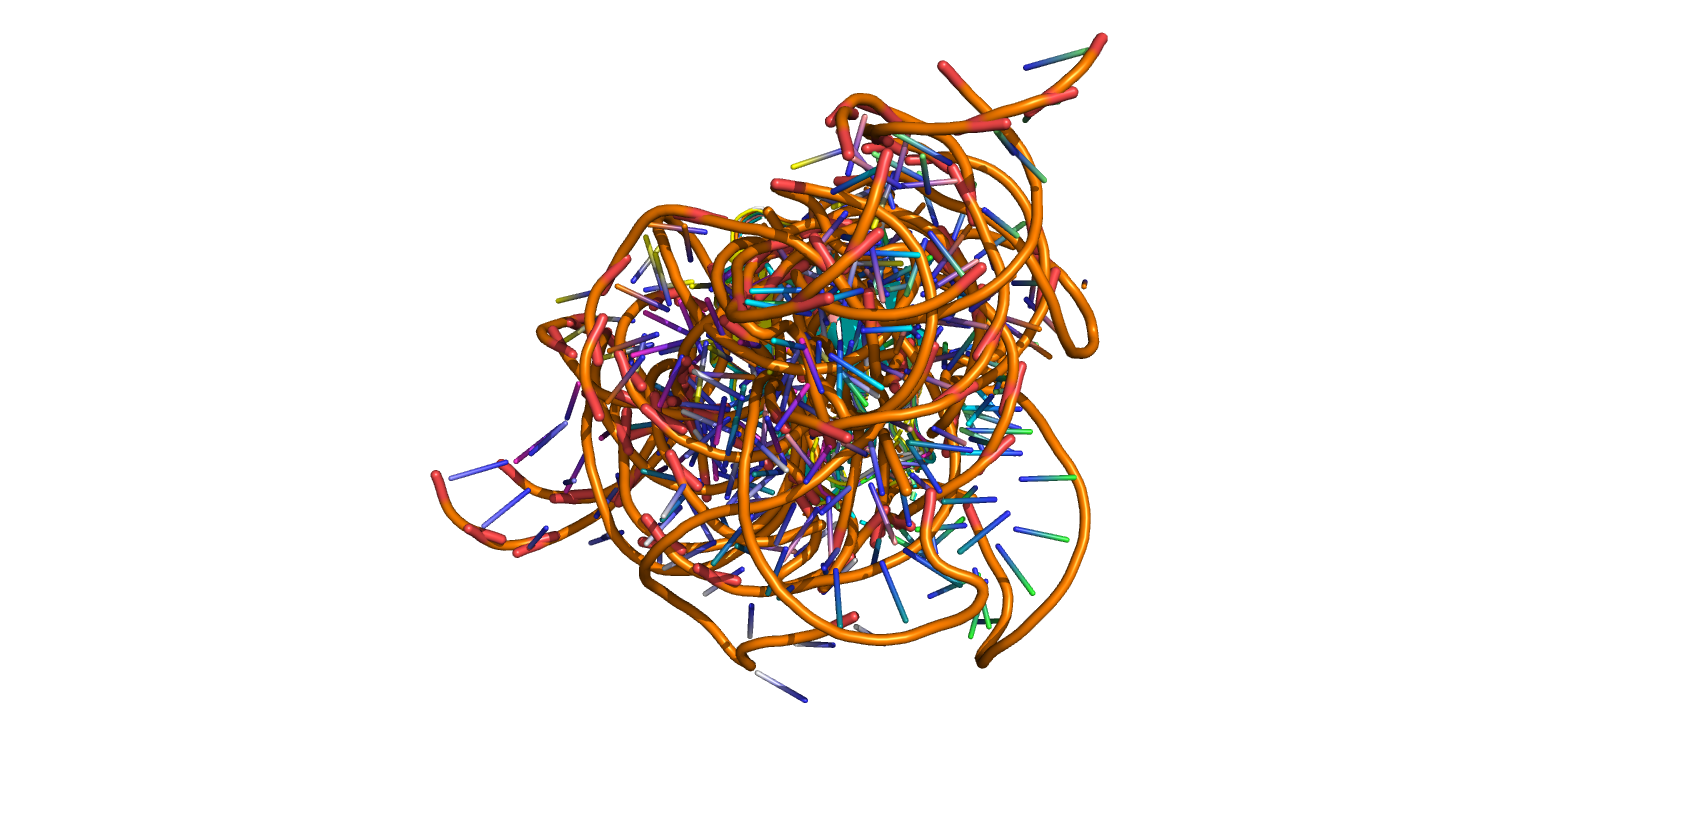
\includegraphics[width=0.9\linewidth]{assets/RMM1_mut2_ALL.png}
% \end{center}

% Podemos observar que los modelos difieren muchísimo entre sí. Parece ser que la mutación desestabiliza la interacción.  Visualizado con \href{https://pymol.org/2/}{\texttt{Pymol}}.

% \subsection*{Anexo K: Visualización de los 10 mejores modelos de docking entre MSI-1 y el RNA mutante 3}\label{anexo_K}
% \addcontentsline{toc}{subsection}{Anexo K: Visualización de los 10 mejores modelos de docking entre MSI-1 y el RNA mutante 3}

% \begin{center}
%     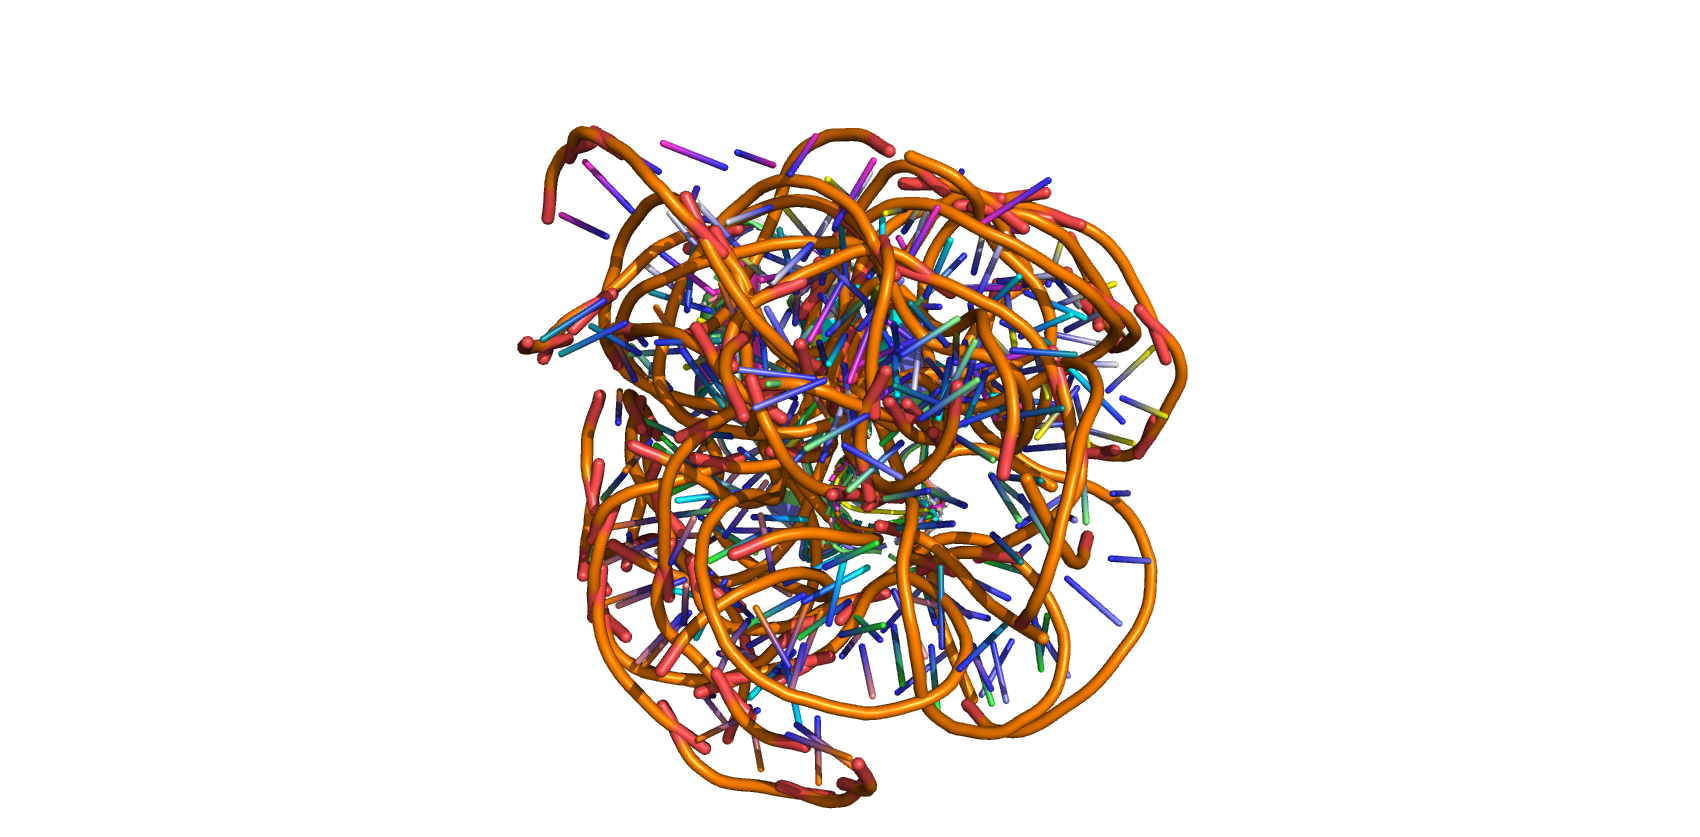
\includegraphics[width=0.9\linewidth]{assets/RMM1_mut3_ALL.png}
% \end{center}

% Podemos observar que los modelos difieren muchísimo entre sí. Parece ser que la mutación desestabiliza la interacción.  Visualizado con \href{https://pymol.org/2/}{\texttt{Pymol}}.

% \subsection*{Anexo L: Visualización de los 10 mejores modelos de docking entre MSI-1 y el RNA mutante 4}\label{anexo_L}
% \addcontentsline{toc}{subsection}{Anexo L: Visualización de los 10 mejores modelos de docking entre MSI-1 y el RNA mutante 4}

% \begin{center}
%     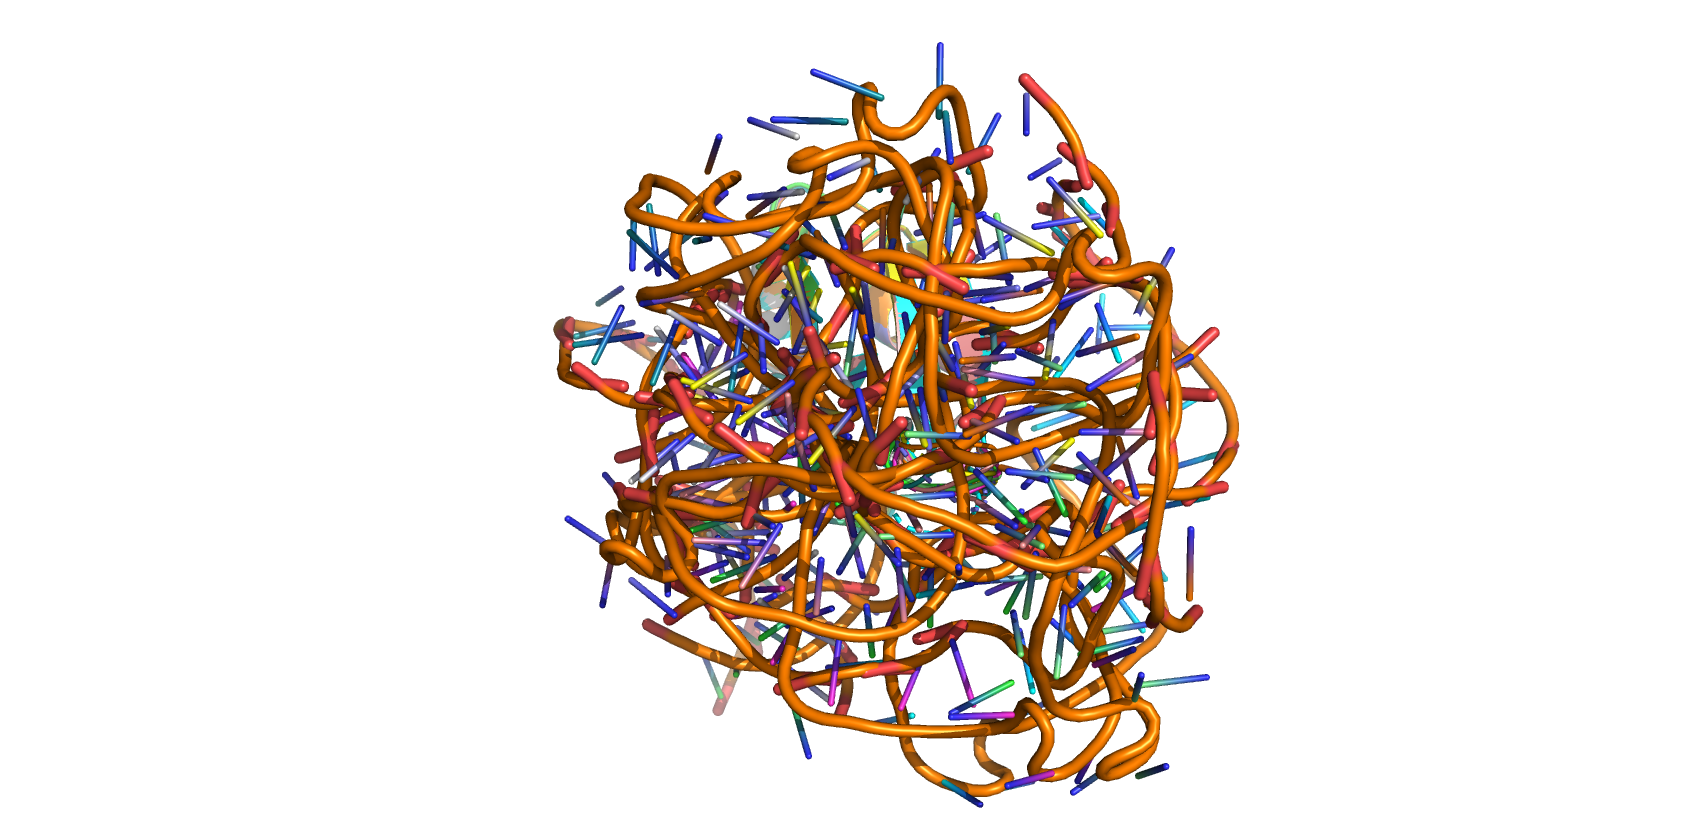
\includegraphics[width=0.9\linewidth]{assets/RMM1_mut4_ALL.png}
% \end{center}

% Podemos observar que los modelos difieren muchísimo entre sí. Parece ser que la mutación desestabiliza la interacción.  Visualizado con \href{https://pymol.org/2/}{\texttt{Pymol}}.

% \subsection*{Anexo M: Visualización de los 10 mejores modelos de docking entre MSI-1 y el RNA mutante 5}\label{anexo_M}
% \addcontentsline{toc}{subsection}{Anexo M: Visualización de los 10 mejores modelos de docking entre MSI-1 y el RNA mutante 5}

% \begin{center}
%     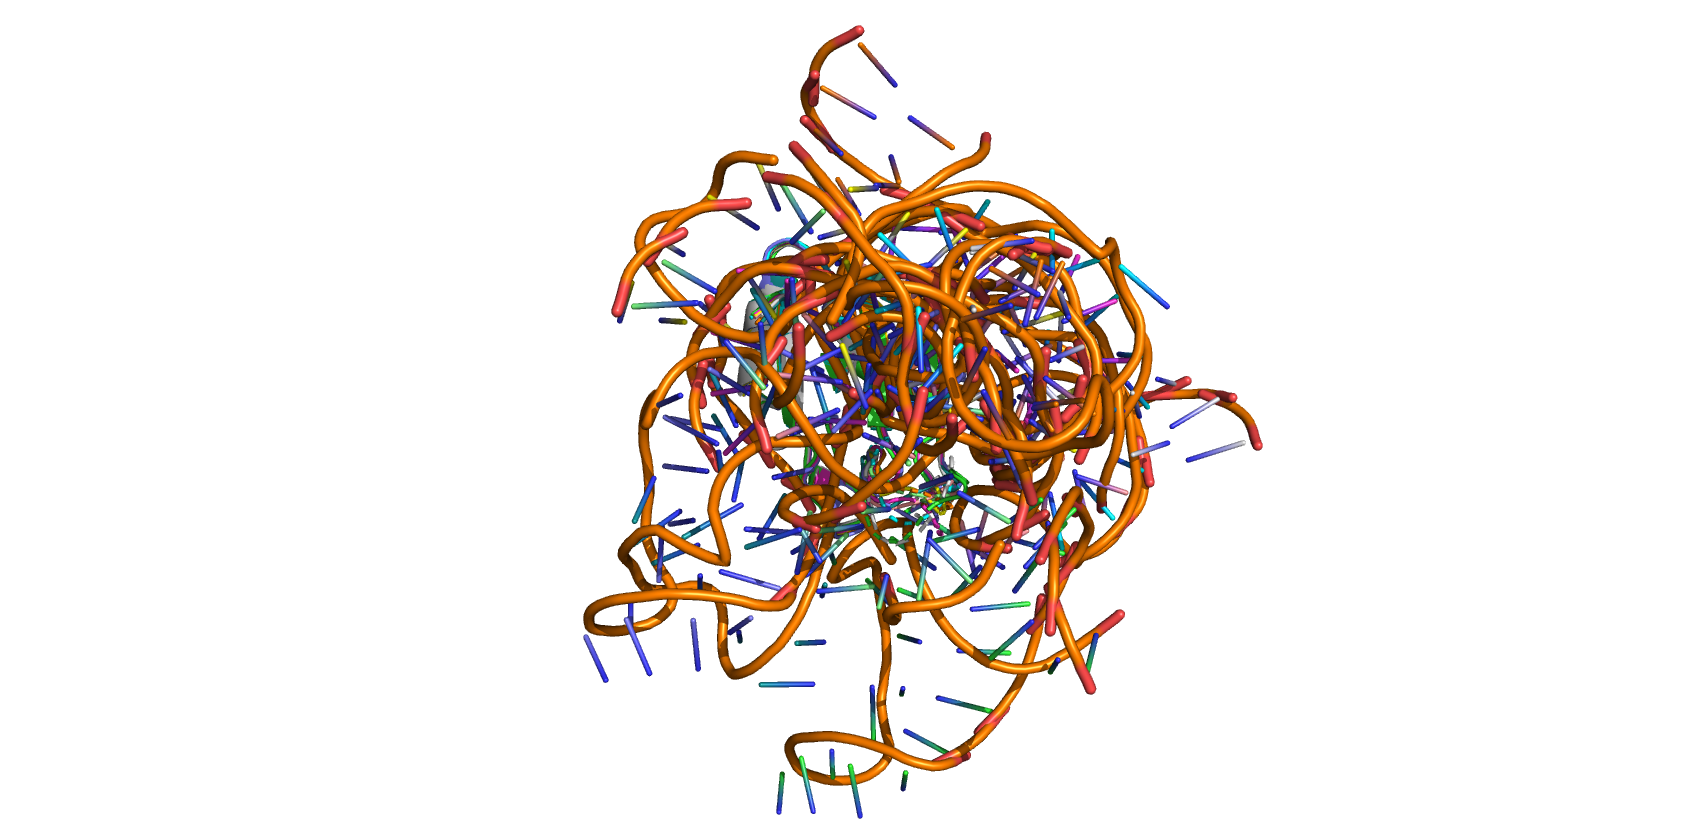
\includegraphics[width=0.9\linewidth]{assets/RMM1_mut5_ALL.png}
% \end{center}

% Podemos observar que los modelos difieren muchísimo entre sí. Parece ser que la mutación desestabiliza la interacción.  Visualizado con \href{https://pymol.org/2/}{\texttt{Pymol}}.

% \subsection*{Anexo N: Tabla de scores para los 10 mejores modelos de cada experimento de docking}\label{anexo_N}
% \addcontentsline{toc}{subsection}{Anexo N: Tabla de scores para los 10 mejores modelos de cada experimento de docking}

% \lstinputlisting{assets/allScores.table}

% \subsection*{Anexo O: Visualización de los 10 mejores modelos de docking entre MSI-1 y el RNA original en estructura lineal (sin estructura secundaria)}\label{anexo_O}
% \addcontentsline{toc}{subsection}{Anexo O: Visualización de los 10 mejores modelos de docking entre MSI-1 y el RNA original en estructura lineal (sin estructura secundaria)}

% \begin{center}
%     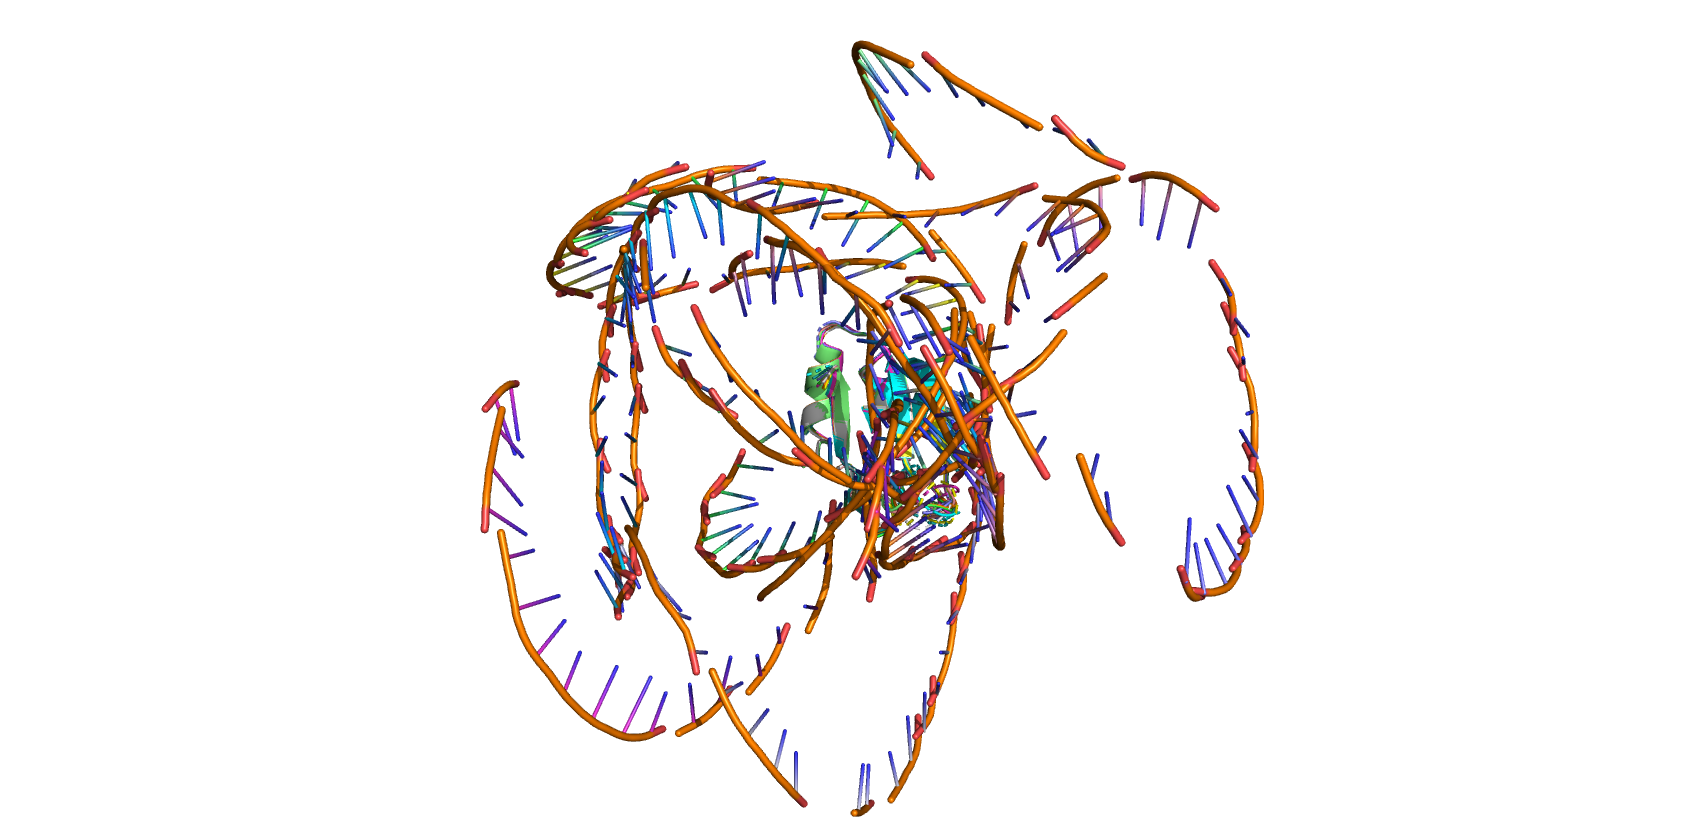
\includegraphics[width=\linewidth]{assets/linear_no_restraints.png}
% \end{center}

% Podemos observar que los modelos difieren muchísimo entre sí. En comparación con la simulación mediante el RNA con la estructura secundaria adecuada, la estructura lineal da peores resultados. Este resultado es coherente con la naturaleza, puesto que en disolución, el RNA adopta estructuras secundarias para la minimización de su energía libre de Gibbs.  Visualizado con \href{https://pymol.org/2/}{\texttt{Pymol}}.


\end{document}